% --------------------------------------------------------------------------------
% Concepts: Experiments
% --------------------------------------------------------------------------------

% ================================================================================
\chapter{Experiments}
\hypertarget{Chapter:ConceptsExperiments}{}
% ================================================================================

% --------------------------------------------------------------------------------
\section{Introduction}
% --------------------------------------------------------------------------------

\IPEMTBC ...Doublecheck this...

Whereas the previous chapter provided a background and description
of the basic modules contained in the IPEM Toolbox, this chapter
focuses on a comparison of the results obtained with our tools
with these obtained from psychoacoustical experiments. Each of the
sections in this chapter contains:
\begin{itemize}
\item a small introduction in which the purpose of the experiment is explained
\item a description of the method that is used
\item a summary of how to run the experiment in practice using
the toolbox and its functions
\item an overview of the obtained results and a discussion thereof
\end{itemize}
The experiments are explained from a conceptual viewpoint, and
each time a link is made between these concepts and the practical
tools (MATLAB functions) available in the toolbox.\\

The following experiments are included:
\begin{itemize}
\item Simulations of roughness in comparison with psychoacoustical data.
\item Short-term model of tonal induction experiments which apply
contextuality to simulate two psychological experiments.
\end{itemize}
Each experiment can be seen as a comparison of one (or more)
module(s) that were handled in the previous chapter with data
obtained from experiments in the psychoacoustic research field.

% --------------------------------------------------------------------------------
% --------------------------------------------------------------------------------
\newpage
\section{Roughness experiments}
% --------------------------------------------------------------------------------

% Make target for following functions:
\hypertarget{Concepts:IPEMRoughnessDemo}{}
\hypertarget{Concepts:IPEMGenerateANIForRoughnessTest}{}
\hypertarget{Concepts:IPEMGenerateANIForScales}{}
\hypertarget{Concepts:IPEMRoughnessRun}{}

\subsection{Introduction}
% --------------------------------------------------------------------------------
The \hyperlink{Concepts:Roughness Module}{Synchronization Index
Model}, which forms the kernel of the Roughness Module (RM), is
based on the idea that roughness depends on the degree in which
neurons synchronize with the beating frequencies. The model
provides a straightforward visualization of the components
contributing to roughness.

In this demonstration the Roughness Module is compared with
behavioral data in psychoacoustics and music psychology. Due due
the fact that a lot of sounds are processed, this demonstration
consumes time and hard disk memory. The output needs about
253MBytes of your hard disk. Performing the full demonstration
takes about 29 minutes on a Windows NT 4.0 system with Pentium
III 600 MHz processor, 256Mb RAM PC130.

% --------------------------------------------------------------------------------
\subsection{Method}
% --------------------------------------------------------------------------------

\IPEMTBC

%\subsubsection*{Framework}
%% --------------------------------------------------------------------------------
%The synchronization index model involves two concepts of
%band-pass filtering:
%\begin{itemize}
%\item
% A concept related to the resonance
%properties of the basilar membrane (=cochlear mechanical
%filtering).
% The width of the band-pass filters that simulate the
%resonance properties simulate the excitation on the basilar
%membrane. The equal width of excitation along the membrane
%corresponds to a quasi-logarithmic relationship in the frequency
%domain. We adopted the Auditory Peripheral Module from Van
%Immerseel and Martens \cite{VanImmerseel:92} but any model of the
%auditory periphery can be used in principle provided that it
%transforms sound into rate-code patterns at the level of the
%auditory nerve. The essential feature of the peripheral model is
%that it introduces the low frequencies in to the spectrum (owing
%to wave rectification).
%\item
%A type of band-pass filtering related to the synchronization of
%neurons to particular frequencies.\
% The upper limit of synchronization in the auditory nerve, which was implemented in
%the Auditory Peripheral Module at 1250 Hz, is clearly too high to
%account for sensory dissonance and roughness. Conceptually,
%synchronization can be divided into three regions corresponding
%to loudness (from 0 to about 25 Hz), to roughness and sensory
%dissonance (from 25 to about 300 HZ), and to pitch (roughly from
%300 to 1250 Hz). The synchronization model has a focus on the
%region between 25 to 300 Hz, which is known to be the frequency
%region of roughness.
%\end{itemize}
%
%The synchronization index model then calculates the roughness by
%a Fourier analysis of the beating frequency range and summing the
%normalized Fourier (magnitude-related) coefficients that
%represent the modulation depth of the beating frequencies. A
%global range for beating frequencies, however, cannot be
%maintained in all auditory channels. In particular, the
%synchronization filtering seems to rely on more narrow band-pass
%filters in the auditory channels whose central frequency is $<$
%800 Hz.


\subsection{Application}
% --------------------------------------------------------------------------------
\subsubsection*{Some Practical Considerations}
% --------------------------------------------------------------------------------
The contents and the functions of the demonstration package for
the roughness experiments can be found in the directory
IPEM$\backslash$Demos$\backslash$Roughness. To perform the
experiments execute the main script
\hyperlink{FuncRef:IPEMRoughnessDemo}{IPEMRoughnessDemo} for
demonstrating the calculation methods of roughness. The function
\hyperlink{FuncRef:IPEMGenerateANIForRoughnessDemo}{IPEMGenerateANIForRoughnessDemo}
generates all the files for the tests contained in the roughness
demo:
\begin{itemize}
\item
\hyperlink{FuncRef:IPEMGenerateANIForRoughnessTest}{IPEMGenerateANIForRoughnessTest}
(IPEMGenerateANIForRoughnessDemo Part I) generates sounds and
auditory nerve images for the psychoacoustical tests. The sounds
and images are further processed with IPEMRoughnessDemo (Part II).

\item
\hyperlink{FuncRef:IPEMGenerateANIForScales}{IPEMGenerateANIForScales}
(IPEMGenerataANIForRoughnessDemo Part II) generates an ANI and
soundfile of several harmonic and inharmonic sounds for the
musical tests.
\end{itemize}

The output, a number of mat-files containing the required auditory
nerve images and the soundfiles, is stored in the directory
RoughnessDemo relative to IPEMRootDir ('output').  The function
\hyperlink{FuncRef:IPEMRoughnessRun}{IPEMRoughnessRun} then calculates roughness of all the specified auditory nerve images using
different models and parameters.

\subsubsection*{Psychoacoustical tests}
% --------------------------------------------------------------------------------
This section compares the model's output with psychoacoustical
data. We start with amplitude modulated signals because they are
characterized by a few parameters whose effect of roughness has
been studied by many authors. We consider the effects of
modulation depth ($m$), amplitude ($A$), carrier frequency
($f_c$), and modulation frequency ($f_m$).

\begin{enumerate}
\item {\textbf{Modulation depth}}
    The dependency of the roughness $R$ on the degree of modulation
    $m$ has been expressed as a power law $R \sim m^n$. Depending on
    the experimental setup, $n$ can slightly vary from $1.2$ up to
    about $2$ \cite{Terhardt:97}. Figure (\IPEMTBC ask Marc)
    \ref{Fig:RoughnessExperimentsModulationDepth} shows the roughness of an amplitude
    modulated tone with $f_c$ 1000 Hz, $f_m$70 Hz, 60 dB in function
    of the modulation depth $m$ linearly increasing from 0 to 1.
    \begin{figure}[h]
        \centering
        
\includegraphics[width=\IPEMDefaultFigureWidth]{Graphics/MissingFigure}
        \caption{Calculated roughness as a function of modulation index $m$ =
        0...1 for a 1000 Hz AM tone}\label{Fig:RoughnessExperimentsModulationDepth}
    \end{figure}
    The dotted line shows the relation $R \sim m^{1.3}$ for $m \leq
    1$. The slope of this curve depends on the parameter $\delta$
    (see Equation \ref{normalizedRoughness}) which was set to 1.5 to obtain
    this result. A change of $\delta$ has a slight effect on the
    slope of the curve in Fig.~\ref{Fig:RoughnessExperimentsModulationDepth}.

\item {\textbf{Amplitude}}
    The effect of amplitude is illustrated in Fig.~\ref{Fig:RoughnessExperiments6}
    using an AM tone with $f_c$ 1000 Hz, $m = 1$, $f_m$ 50 Hz, and a
    linear decrease of SPL dB from 70 to 0. The dynamic range of
    neurons is known to be limited in the order of 30-50 dB. However,
    the large dynamic range of the human auditory system is explained
    by the spread of excitation due to the resonance characteristics
    of the basilar membrane \cite{Smith:88}. The spread of excitation
    is reflected in figure ~\ref{Fig:RoughnessExperiments26}a where a broad excitation
    range can be noticed at a level of 70 dB. This range narrows down
    as the level decreases. In figure ~\ref{Fig:RoughnessExperiments26}b, however, one
    may notice that the excitations contribute to the same frequency
    of 50 Hz. From 70 to about 53 dB the roughness halves.
    \begin{figure}[h]
        \centering
        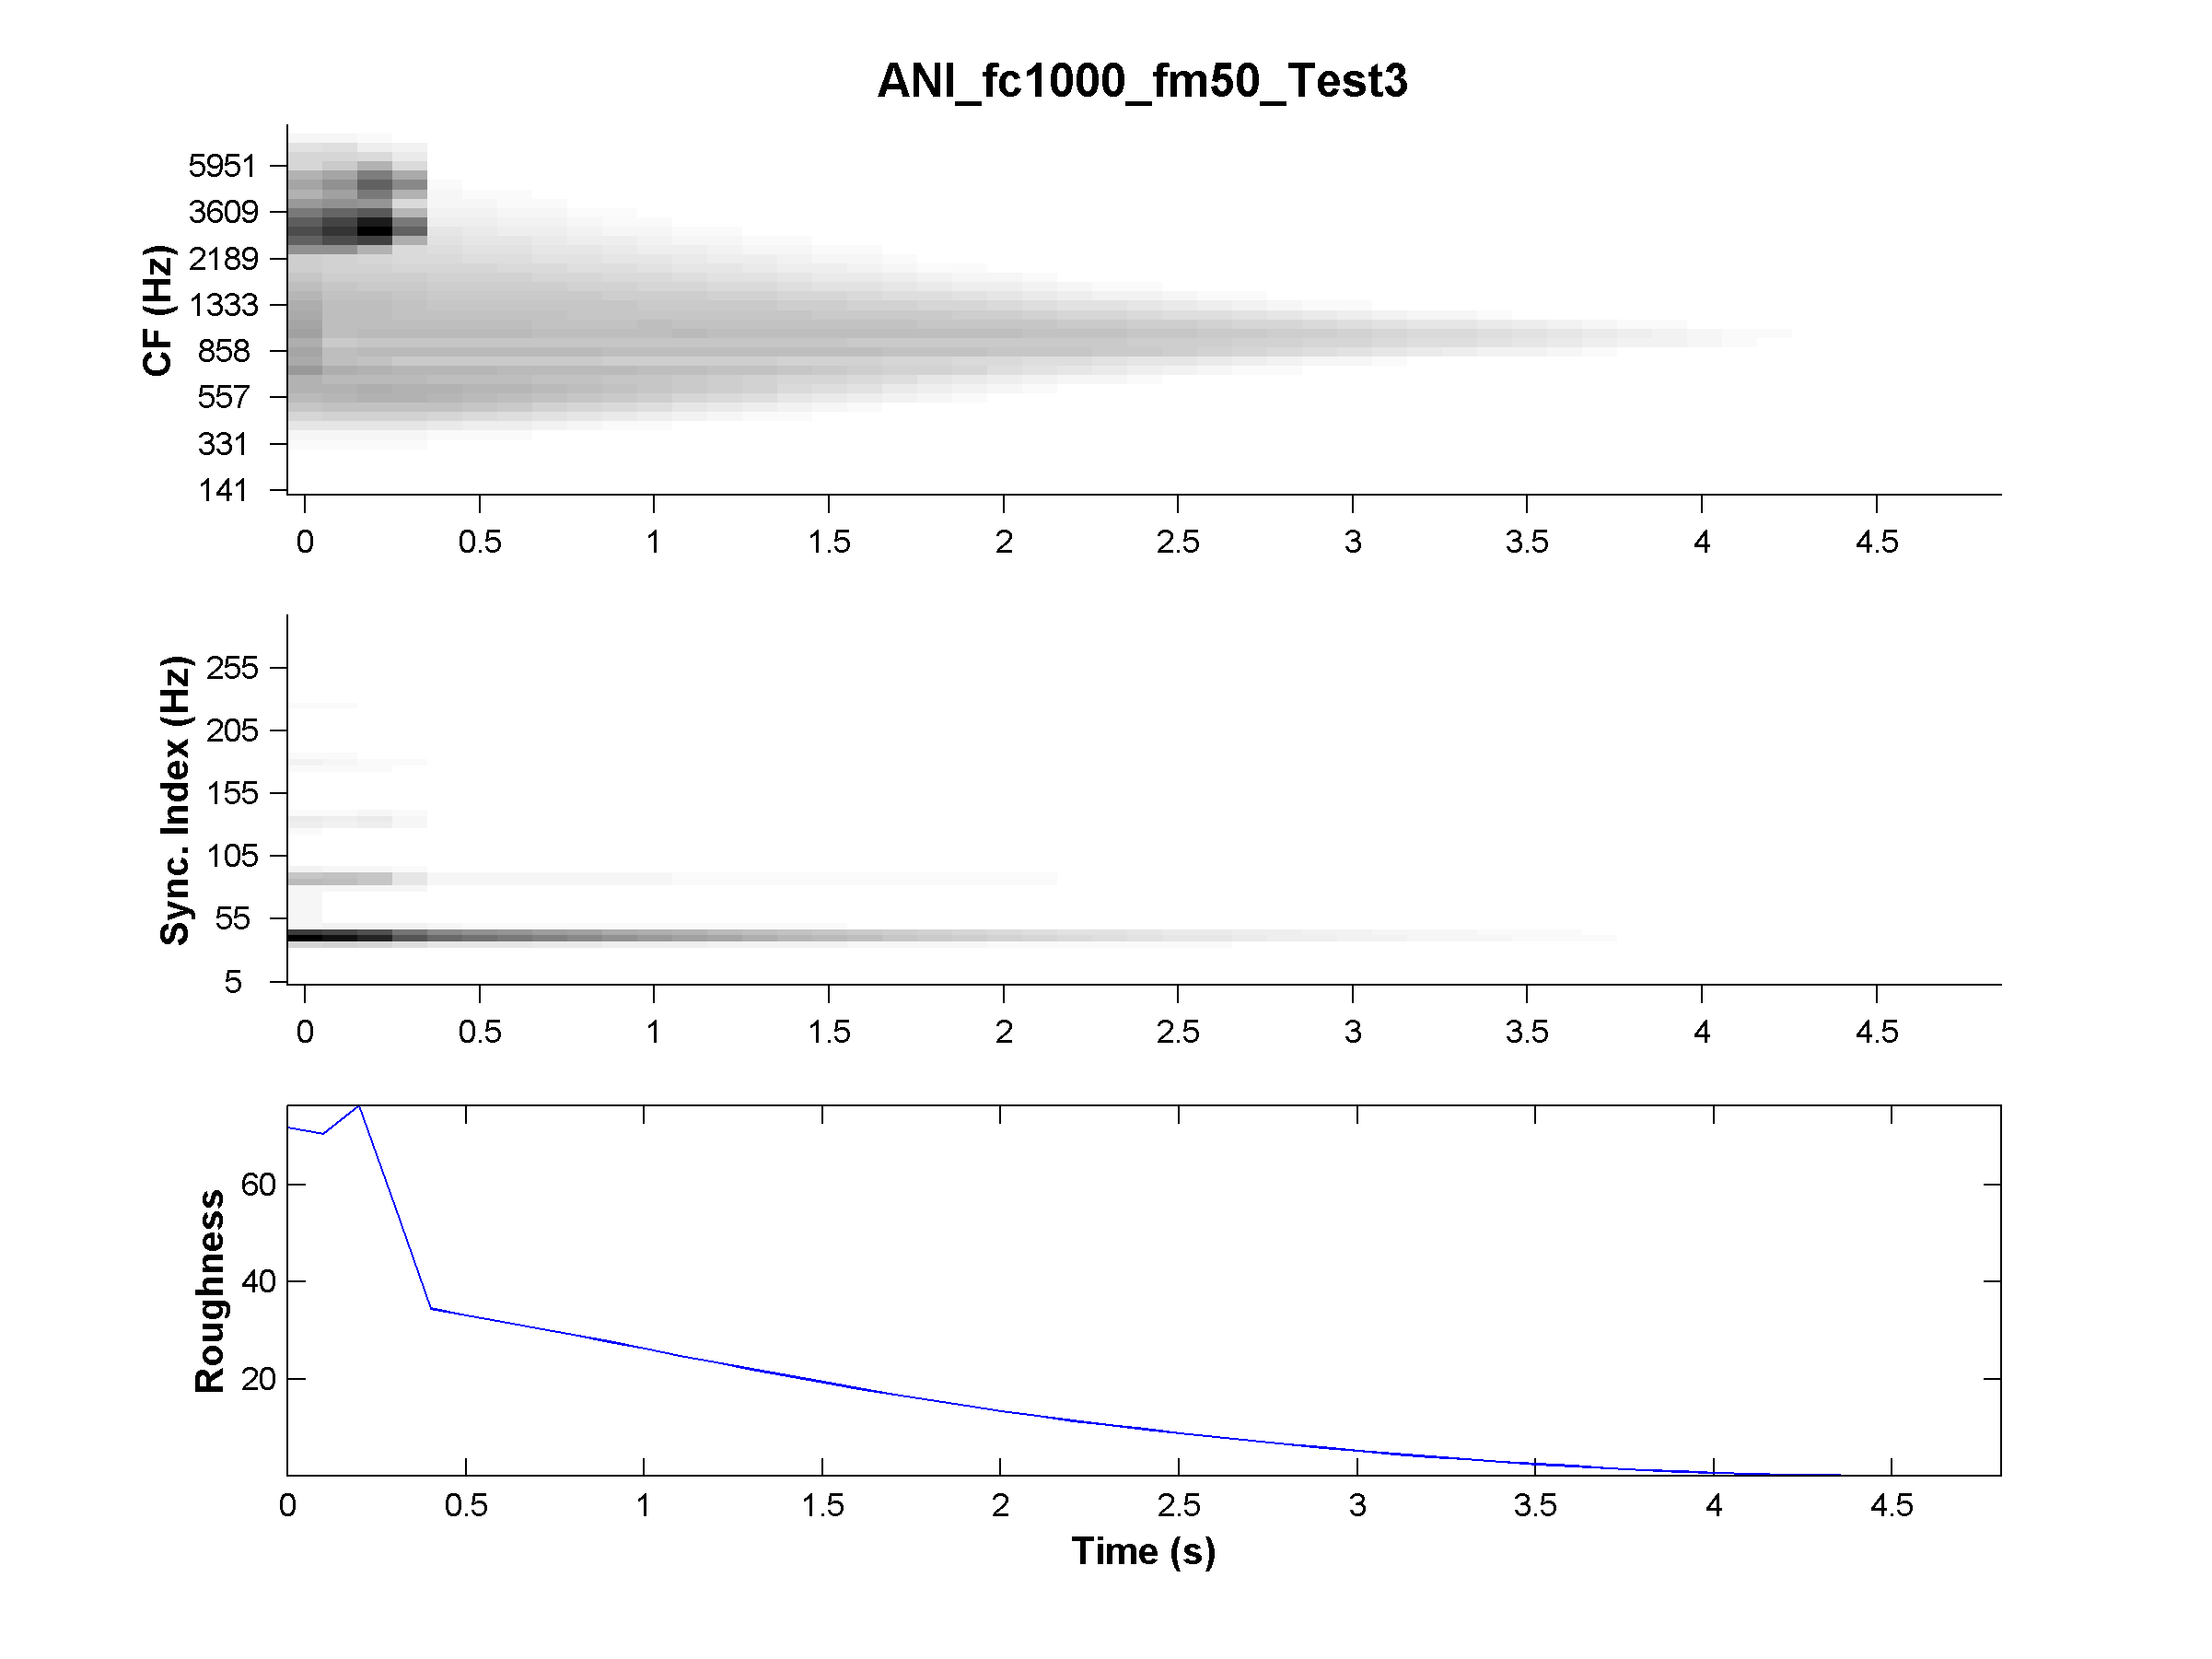
\includegraphics[width=\IPEMDefaultFigureWidth]{Graphics/RoughnessExperiments26}
        \caption{Calculated roughness as a function of amplitude.}
        \label{Fig:RoughnessExperiments26}
    \end{figure}

\item {\textbf{Frequency Modulation}}
    The formula used to calculate an FM tone is
    \cite{DanielWeber:1997}:
    \begin{displaymath}
        s(t) ~=~ \hat{s}.
        sin \left( 2 \pi f_c t - \frac{\Delta f}{f_{mod}}. cos (2 \pi f_{mod} t) \right)
    \end{displaymath}
    where $\hat{s}$ is the effective amplitude. The effects of
    frequency modulation on roughness show a band-pass characteristic
    with maximal values from 40 Hz to 70 Hz \cite{Kemp:1982}
    figure~\ref{Fig:RoughnessExperimentsKemp1}, full line), which our model (dotted line)
    approximates except at $f_{mod}$ 20 Hz, where the estimated
    roughness is clearly too high. The other values fall within the
    quartile range. The signal is
    a 1.6 kHz FM tone at 60 dB with $\Delta f$ 800 Hz whose  roughness
    is measured at $f_{mod}$ 1 10 20 40 60 80 100 200 300 400 500
    Hz.

    \begin{figure}[p]
        \centering
        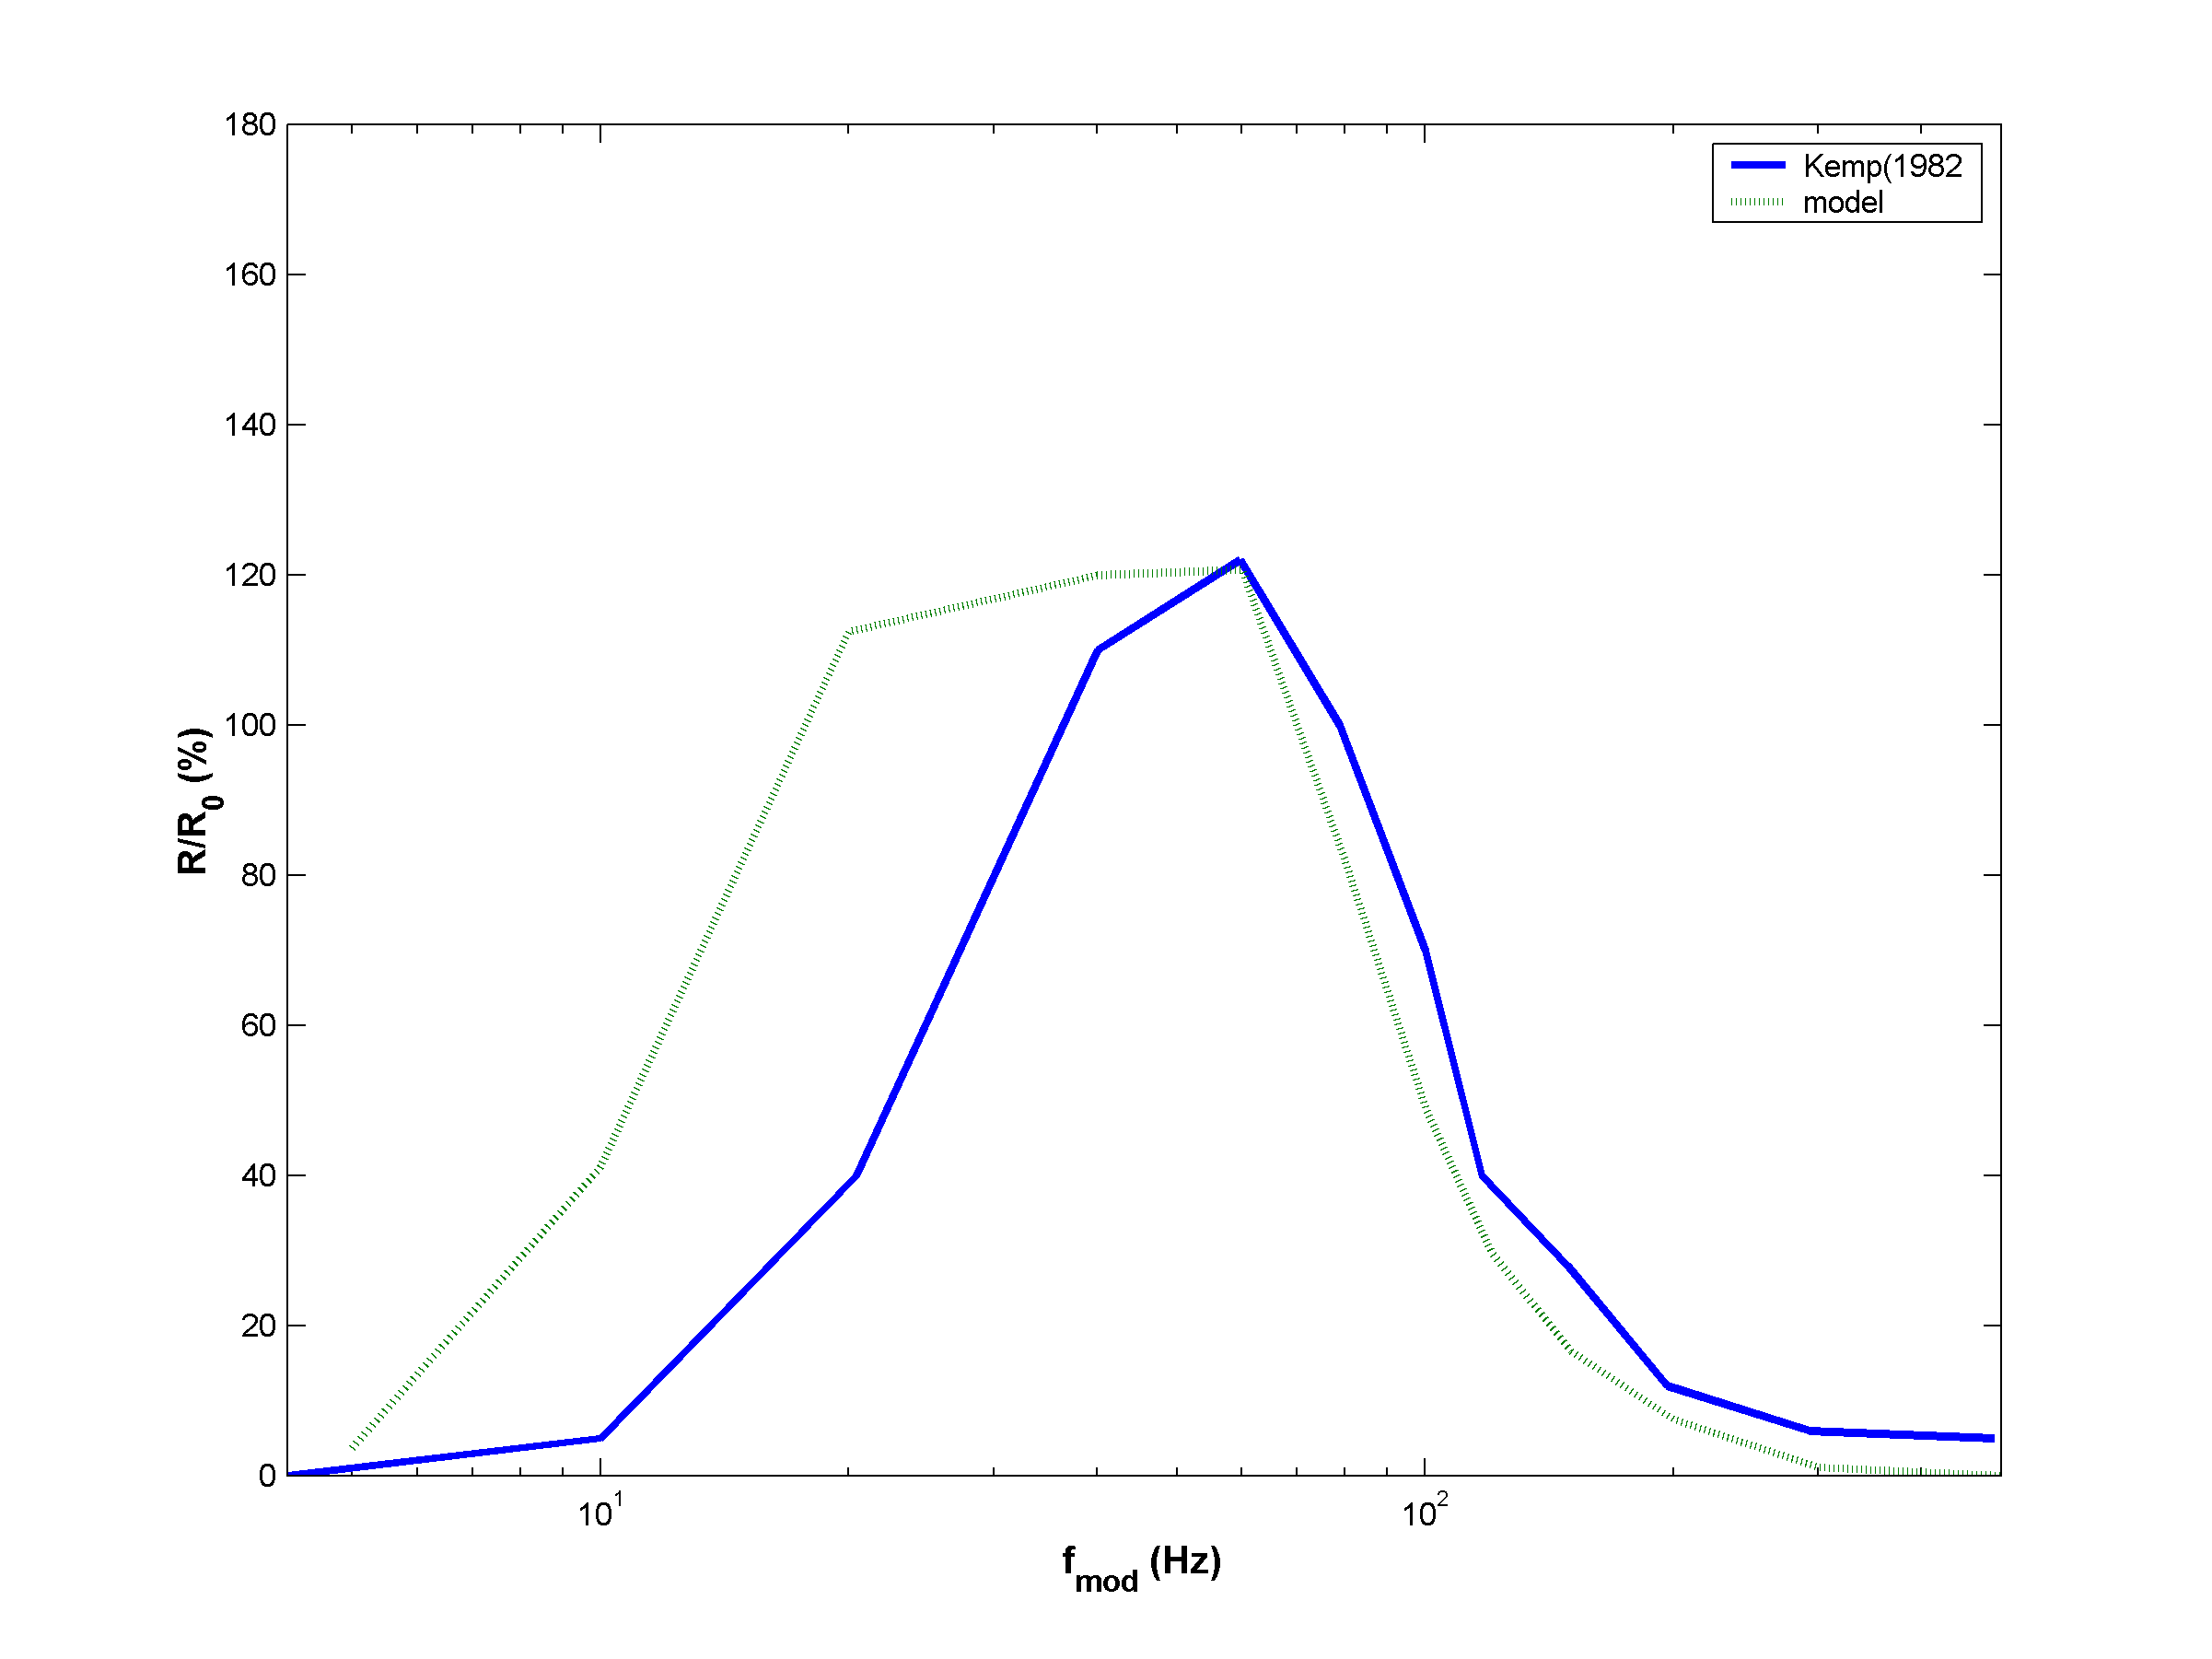
\includegraphics[width=\IPEMDefaultFigureWidth]{Graphics/RoughnessExperimentsKemp1}
        \caption{Calculated roughness as a function of frequency modulation. The signal is
        a 1.6 kHz FM tone at 60 dB with $\Delta f$ = 800 Hz, and $f_{mod}$
        from 1 10 20 40 60 80 100 200 300 400 500 Hz. The peaks are
        generated at the onsets}
        \label{Fig:RoughnessExperimentsKemp1}
    \end{figure}

    In addition, the roughness of a FM tone with $f_c$ 1600 Hz,
    $f_{mod}$ 70 Hz, at 60 dB is measured in function of the frequency
    deviation $\Delta f$ at 10 15 30 60 120 160 340 580 880 1130 1400
    1580 1720 Hz (figure ~\ref{Fig:RoughnessExperimentsKemp2}). The results correspond
    rather well with the available psychoacoustical data, as shown in
    figure ~\ref{Fig:RoughnessExperimentsKemp1}. (All values fall within the quartile
    range).
    \begin{figure}[p]
        \centering
        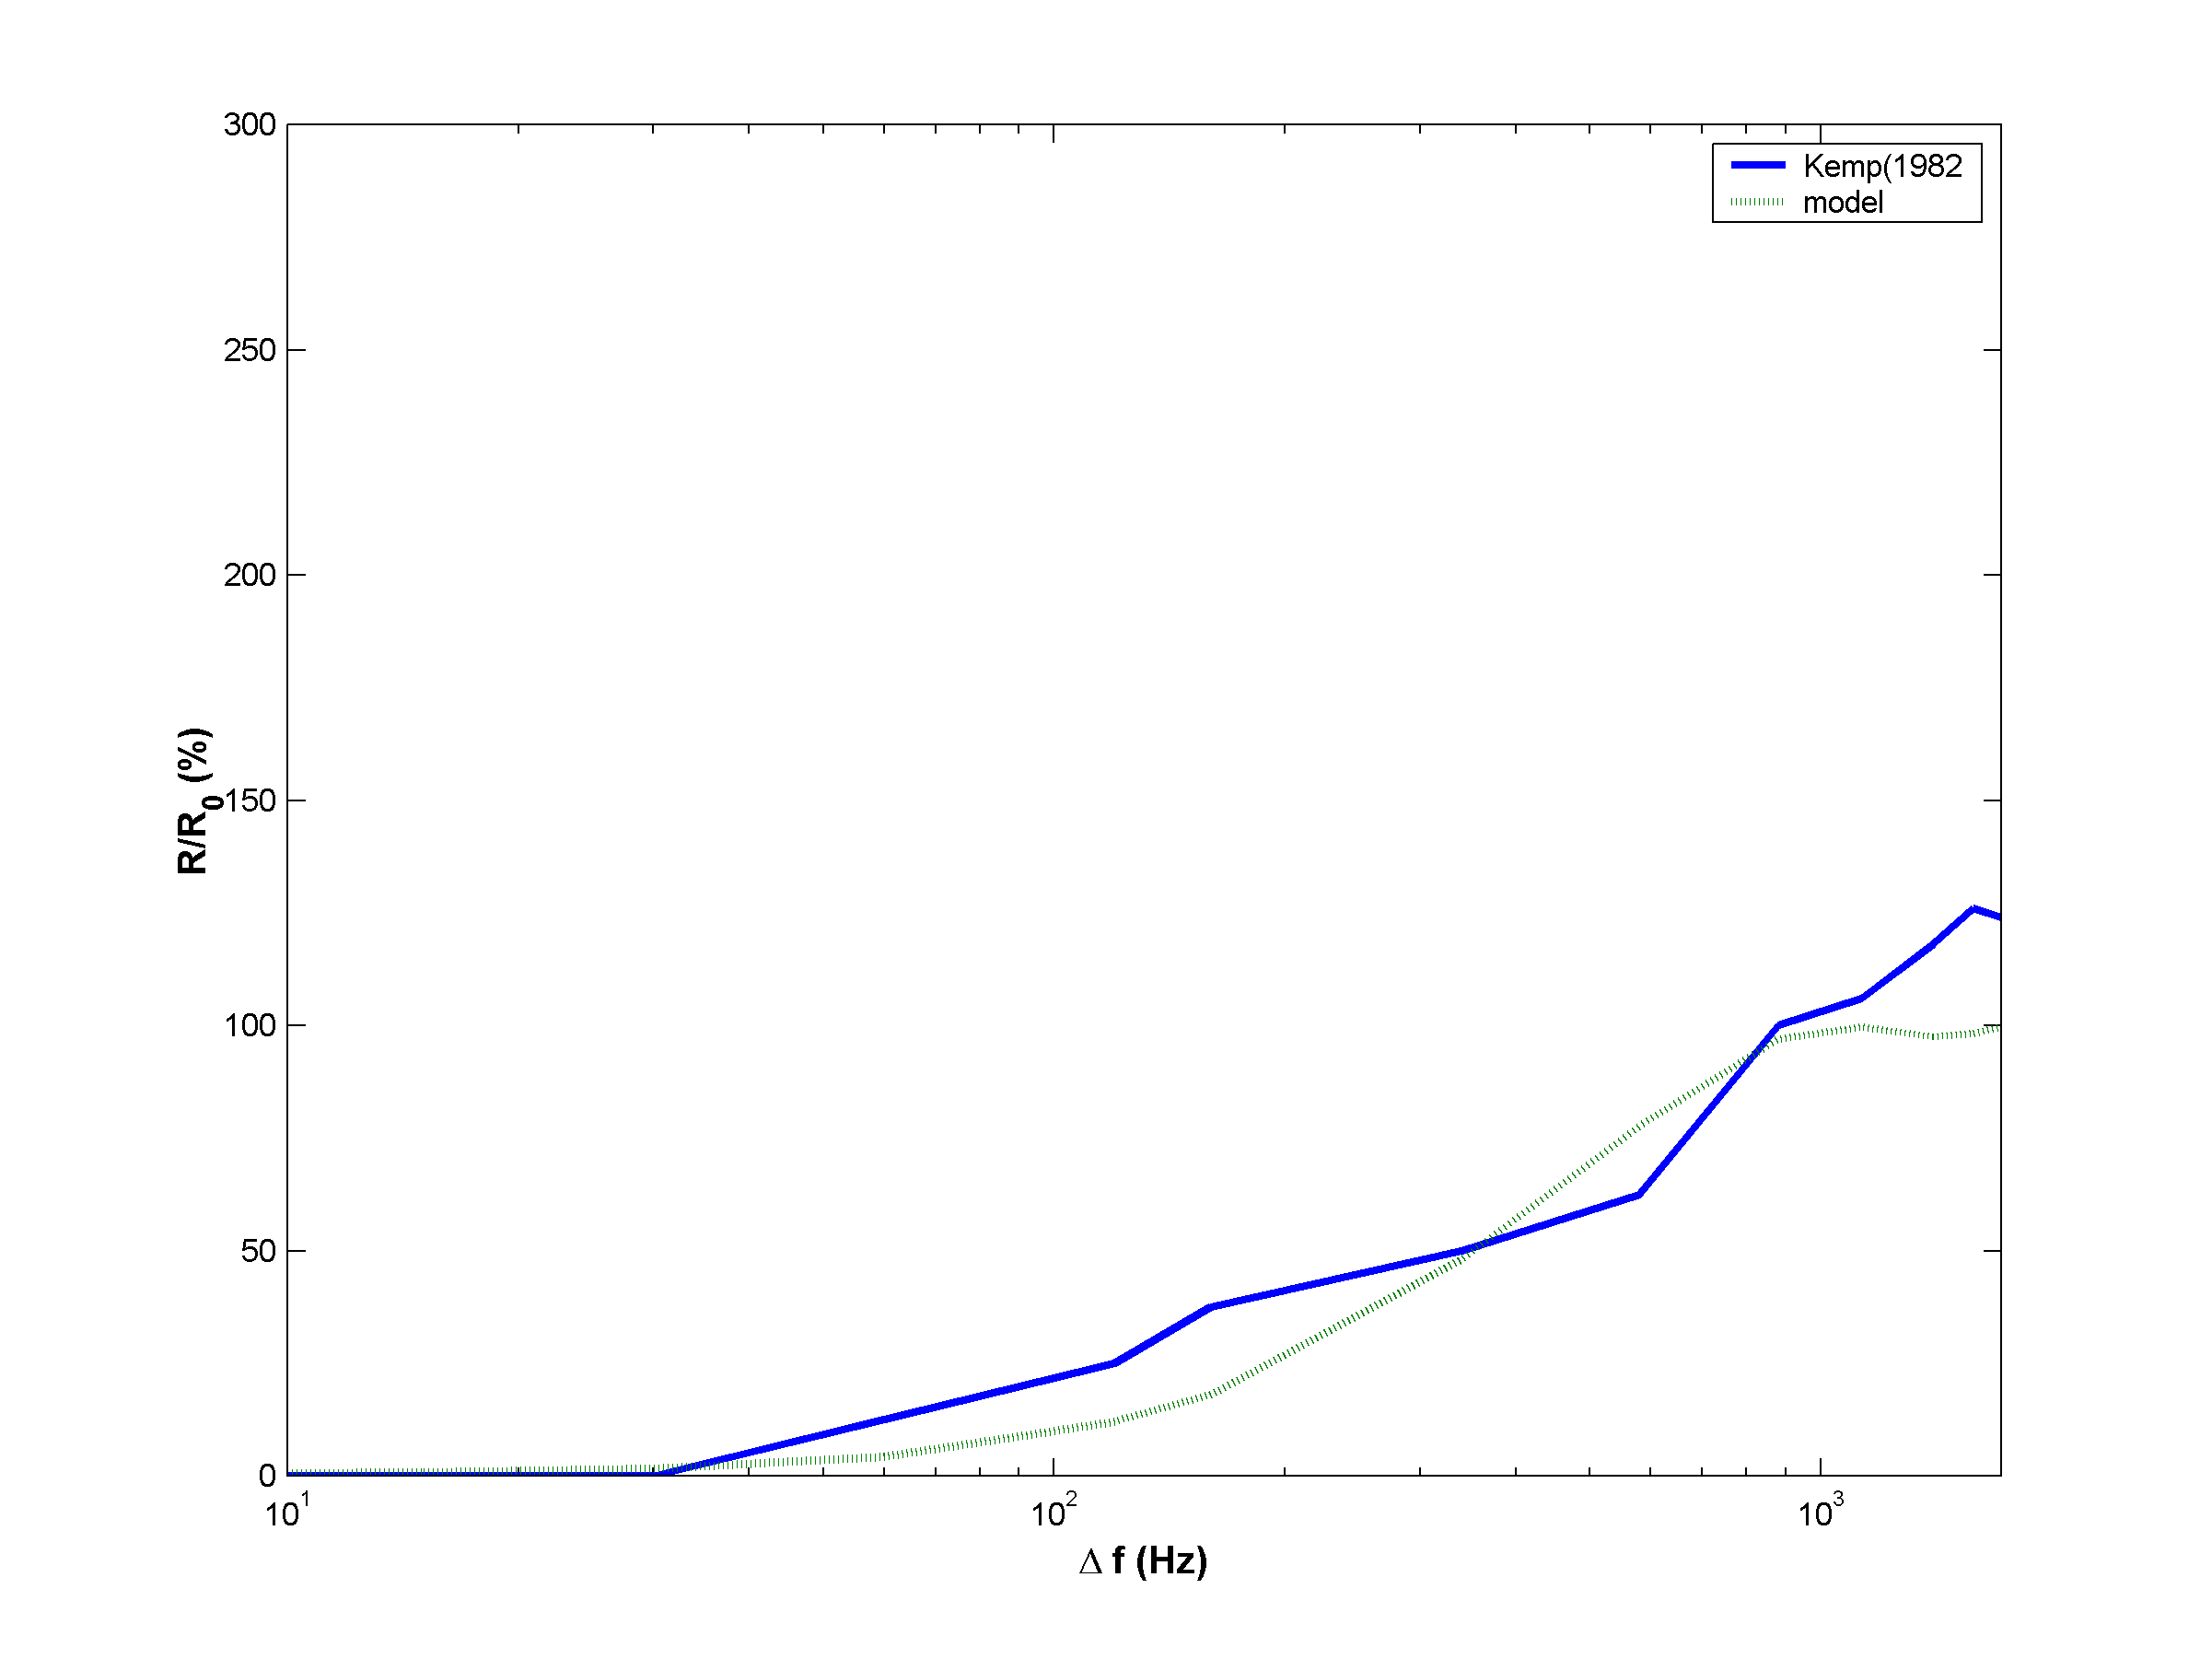
\includegraphics[width=\IPEMDefaultFigureWidth]{Graphics/RoughnessExperimentsKemp2}
        \caption{Comparison of the model's output (dotted line) with
        psychoacoustical data (full line). The signal is
        a 1.6 kHz FM tone at 60 dB with $\Delta f$ 800 Hz measured
        at $f_{mod}$ from 1 10 20 40 60 80 100 200 300 400 500
        Hz.}
        \label{Fig:RoughnessExperimentsKemp2}
    \end{figure}

\end{enumerate}

\subsubsection*{Musical tests}
% --------------------------------------------------------------------------------
The music theoretical interest of the concept of roughness is
demonstrated by taking a harmonic tone complex and playing it
together with a pitch shifted version thus specifying different
musical intervals of the timbre over a defined range. As an
illustration, we took a harmonic tone complex consisting of a
fundamental ($f_0$) at 500 Hz and 5 harmonics with equal
amplitude. This tone is played together with a pitch shifted copy.
The shift over 5 seconds is linear in frequency up to the upper
octave ($f_0$ 1000 Hz). The roughness as calculated with the
synchronization index model is shown in figure
~\ref{Fig:RoughnessExperiments31}.
\begin{figure}[p]
  \centering
  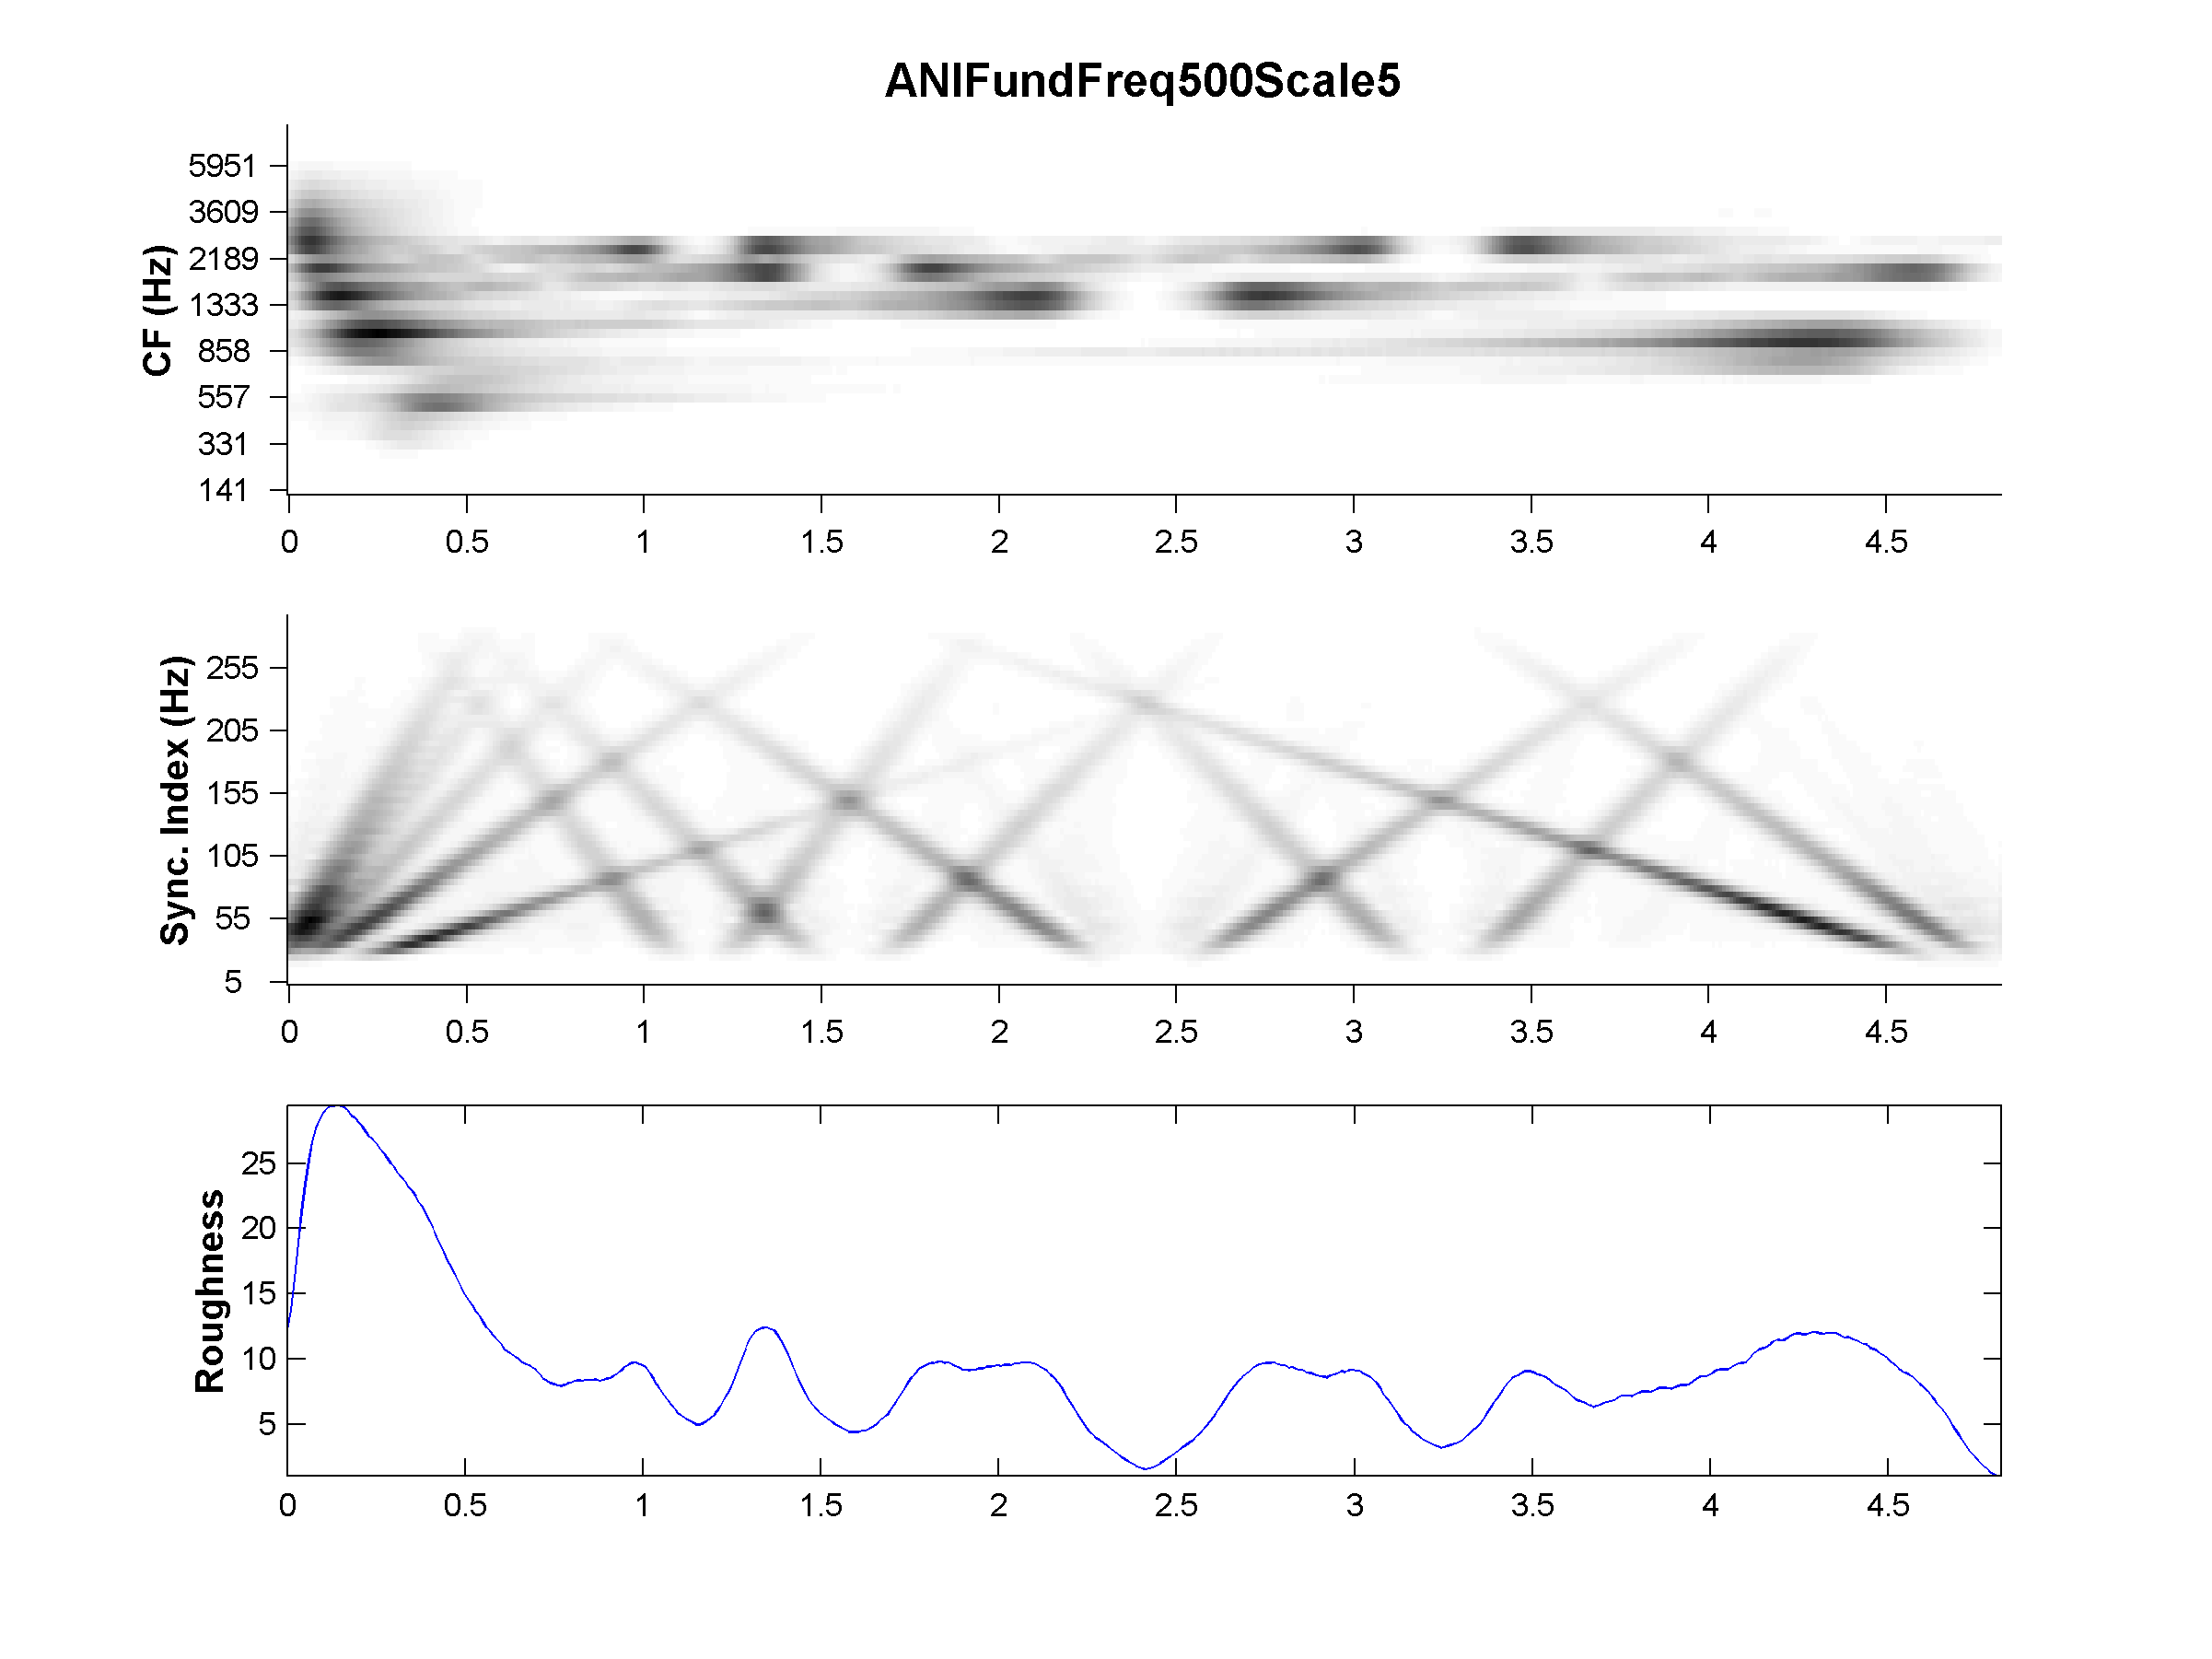
\includegraphics[width=\IPEMDefaultFigureWidth]{Graphics/RoughnessExperiments31}
  \caption{A harmonic tone complex with $f_0$ 500 Hz is played together with a
  pitch shifted copy (up to $f_0$ 1000 Hz). The harmonics have equal amplitudes.
  Top panel: excitation in the auditory channels.  Middle panel: synchronization
  index.
  Lower panel: roughness as calculated with the synchronization index model.}
  \label{Fig:RoughnessExperiments31}
\end{figure}

The roughness curve in figure ~\ref{Fig:RoughnessExperiments31}
can be compared with the results of the curve-mapping model of
roughness of \citeA{Sethares:98}(figure
~\ref{Fig:RoughnessExperiments30}). This model takes the
frequency-amplitude values as input (no sound!) and calculates the
curve using the psychoacoustical curve of \citeA{Plomp}. The
Synchronization Index Model (figure
~\ref{Fig:RoughnessExperiments33}), apart from its good agreement
with this theoretical model, provides an additional cue in showing
the 'spectral' (=excitation in the auditory channels) as well as
'temporal' (=synchronization index profile) factors that
contribute to roughness. Note that the dips are less deep than in
Sethares' model, which is partly due to the fact that the model
works on a glissando of harmonic tone complexes, rather than on
separate intervals. The points of minimal roughness indicate a
hierarchical order of intervals in terms of roughness. This
hierarchy can be musically exploited as the points of minimum
roughness may indicate candidates for a musical scale.

\begin{figure}
    \centering
    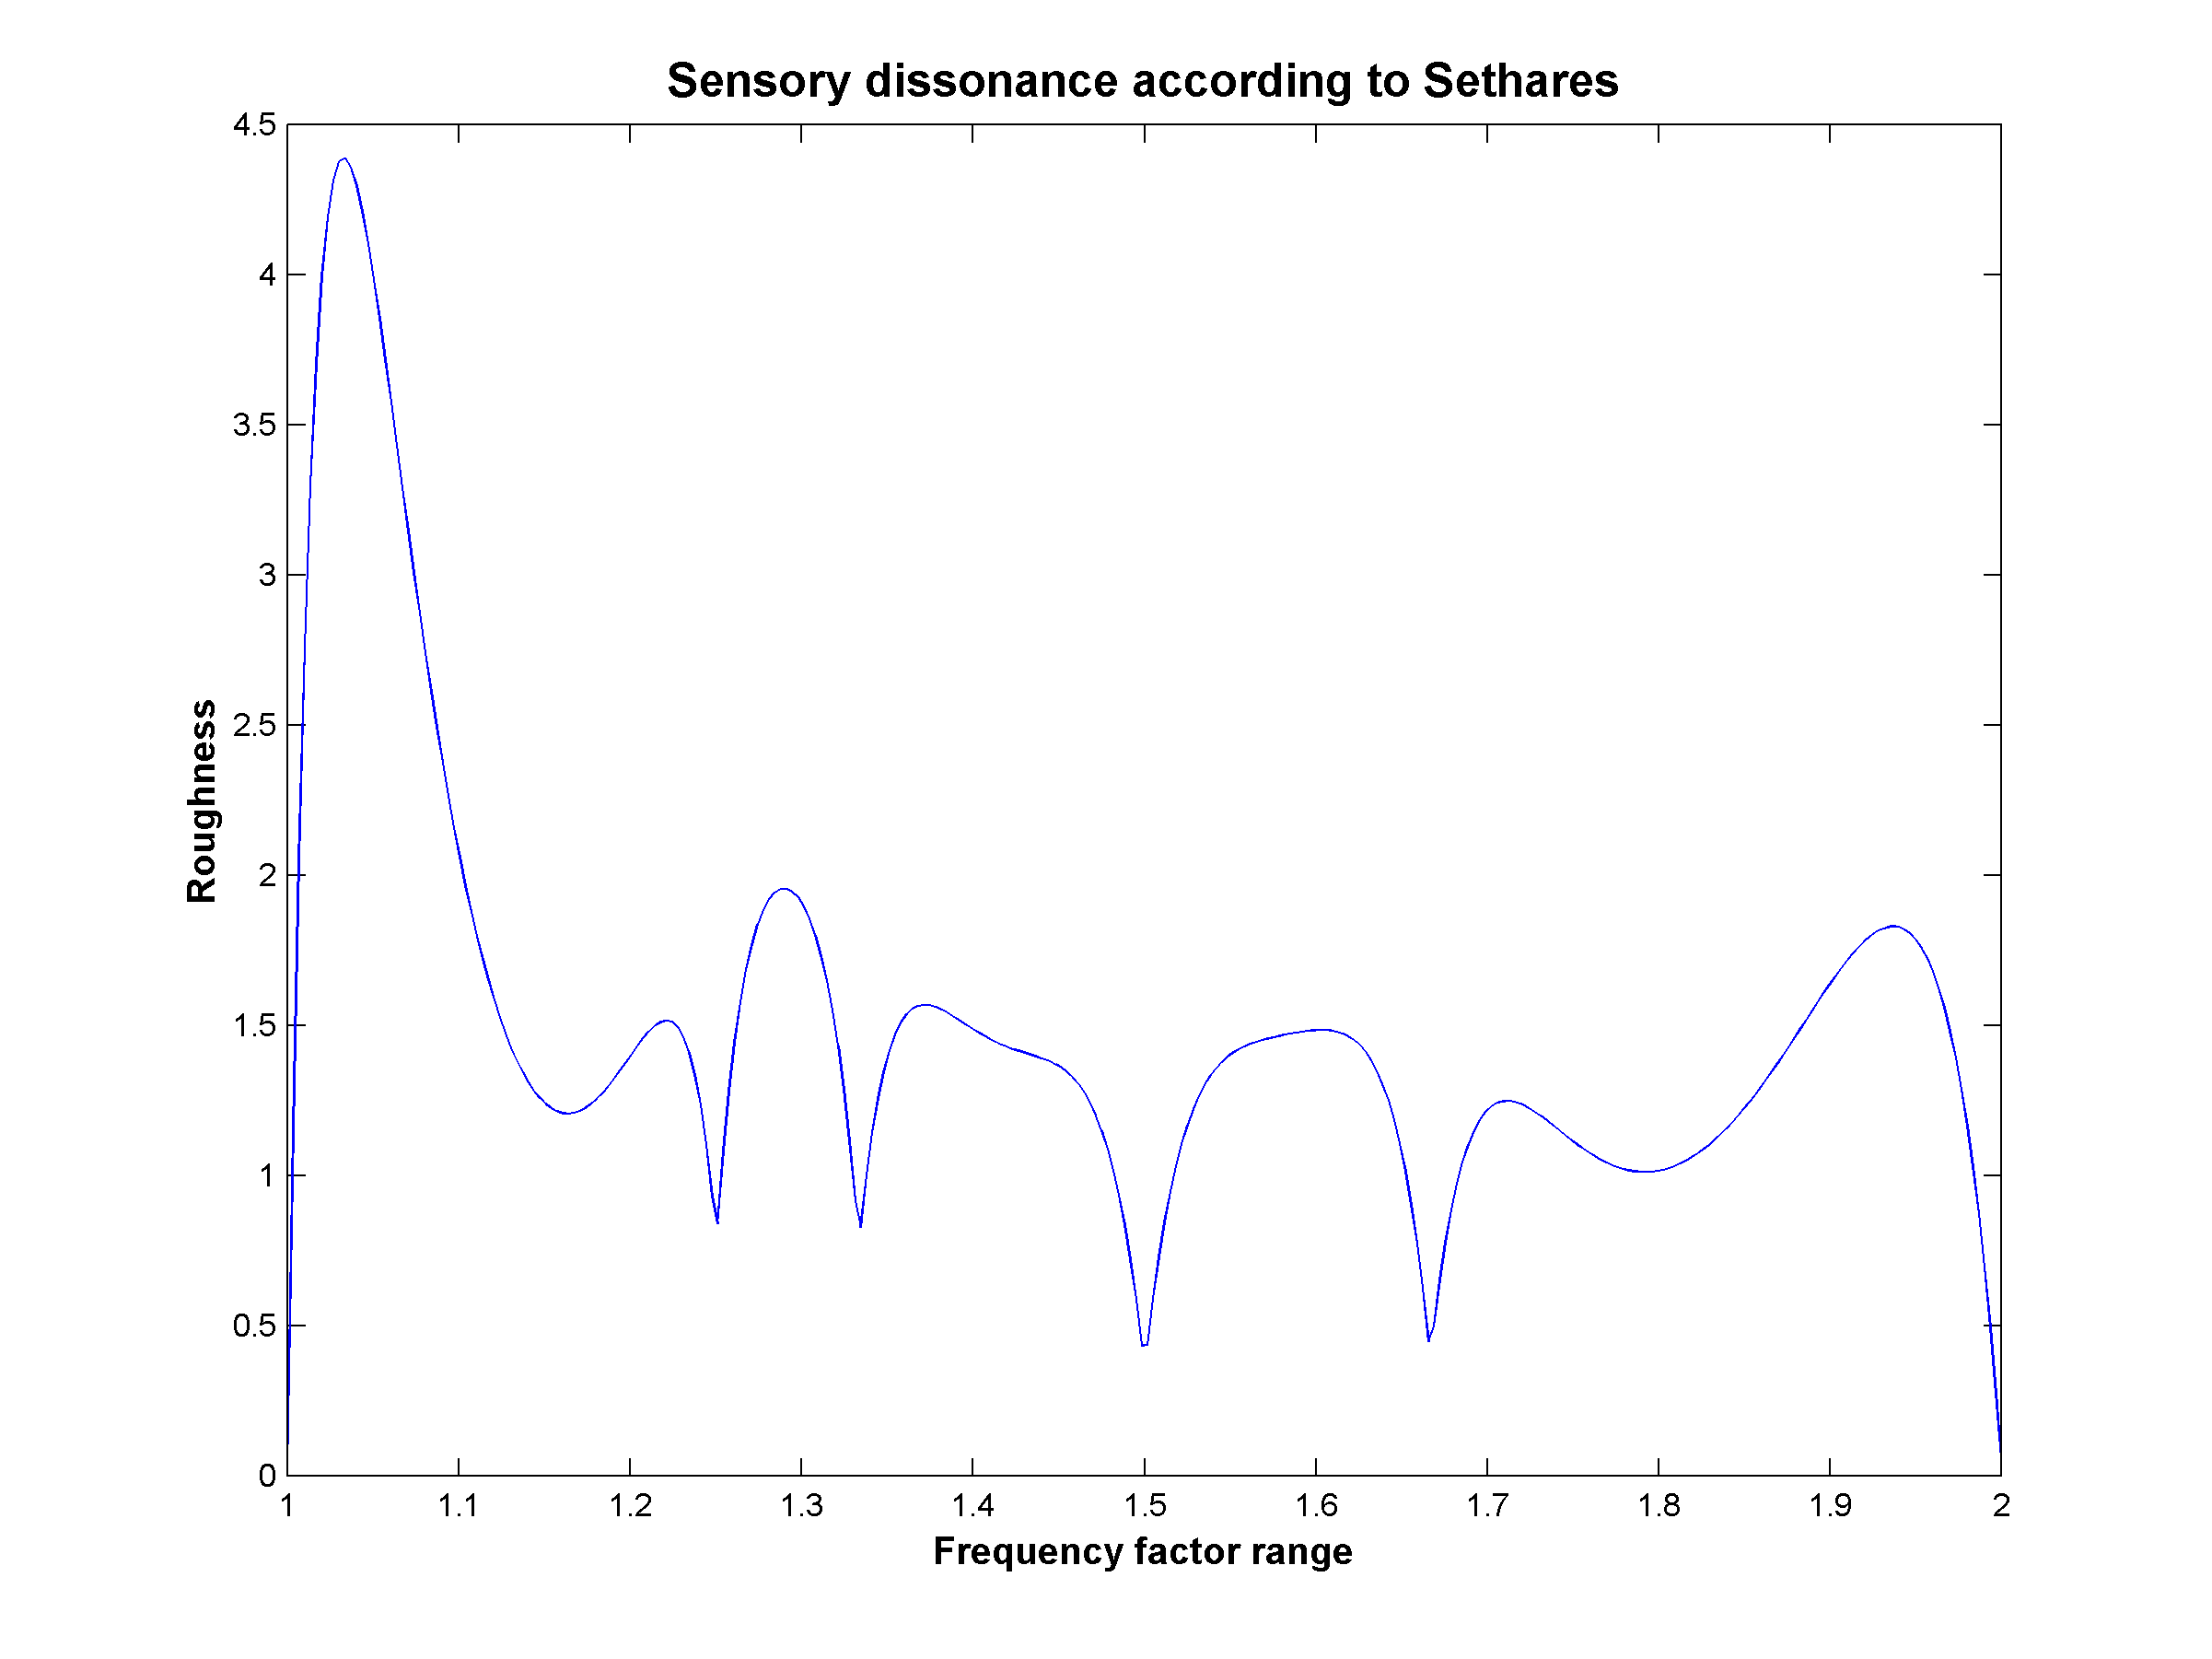
\includegraphics[width=\IPEMDefaultFigureWidth]{Graphics/RoughnessExperiments30}
    \caption{Sensory
    dissonance as calculated with the curve-mapping model of Sethares}
    \label{Fig:RoughnessExperiments30}
\end{figure}

\begin{figure}
    \centering
    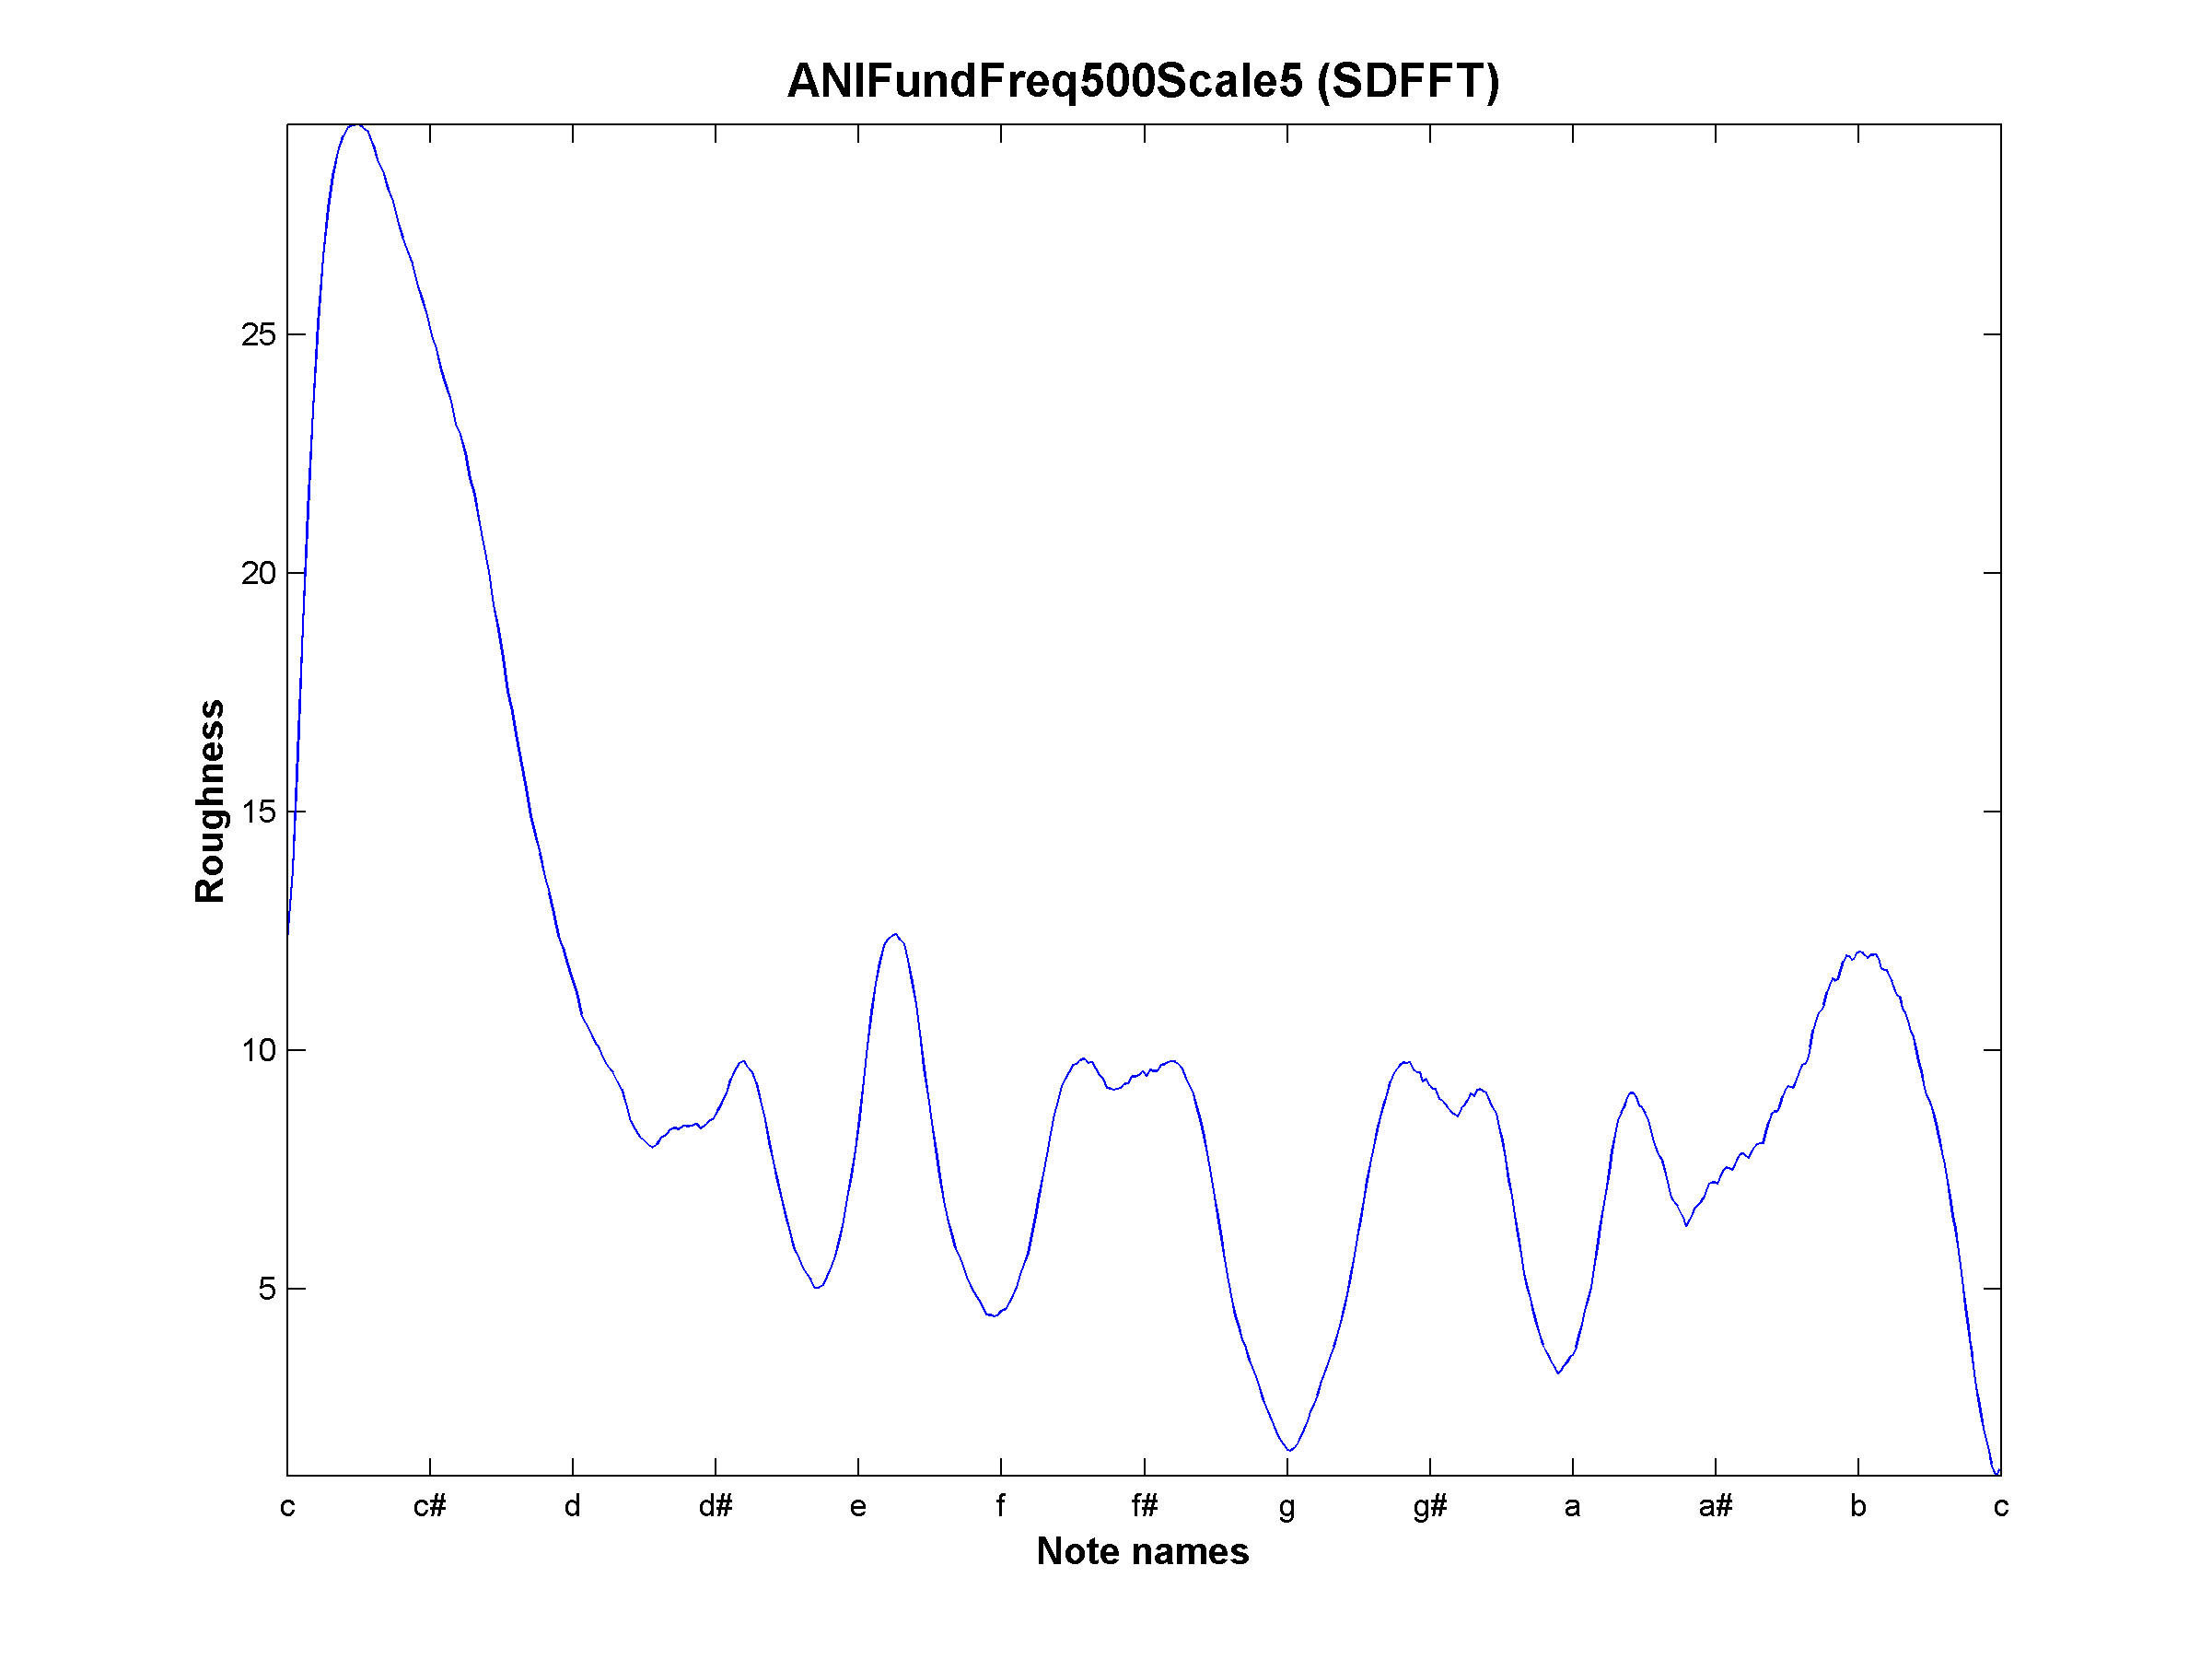
\includegraphics[width=\IPEMDefaultFigureWidth]{Graphics/RoughnessExperiments33}
    \caption{Roughness as calculated with the Synchronization Index Model}
    \label{Fig:RoughnessExperiments33}
\end{figure}

\subsection{Results and discussion}
% --------------------------------------------------------------------------------
\subsubsection*{Dependency}
% --------------------------------------------------------------------------------
The dependency of roughness on $m$, $f_m$ and $f_c$ provides
evidence for the theory that roughness may be directly related to
the degree in which neurons synchronize with the beating
frequencies of the AM tones. Roughness should then depend on two
basic effects:
\begin{itemize}
\item
The 'spectral' filtering resulting from the resonance properties
of the basilar membrane.
\item
The neuronal synchronization and its possible limitations.
\end{itemize}

\subsubsection*{Modulation frequency smaller than 25 Hz}
% --------------------------------------------------------------------------------
For $f_m$ smaller than about 25 Hz, the sensation of roughness
goes over into a sensation of fluctuation and loudness. Roughness
starts at about $f_m > 25 $ Hz but then the effects of spectral
filtering and synchronization should be taken into consideration.

\subsubsection*{Frequencies outside the filter bandwith}
% --------------------------------------------------------------------------------
AM tones have spectral energy at both sides ($f_c \pm f_m$) of a
carrier frequency $f_c$. An increase of the modulation frequency
$f_m$ results in a widening of the intervals. Consequently, when
the side frequencies ($f_c \pm f_m$) fall outside the central
scope of the $f_c$ filter bandwidth, their energy becomes more
and more attenuated and the beating decreases in relation to
that. The bandwidth of the auditory filters corresponds to
resonance regions of equal distance on the basilar membrane
\cite{GreenwoodJoris:1996}. Due to the quasi logarithmic
relationship between distance and frequency, the filter bandwidth
of this filter becomes broader in the higher frequency regions.
The 'spectral' filtering that results from the resonance
properties of the basilar membrane accounts for the fact that the
roughness decreases when $f_m$ exceeds the bandwidth of the
filtering associated with $f_c$. As the frequency components
exceed the bandwidth of an auditory filter, they will no longer
interfere and will cease to produce beating frequencies.

\subsubsection*{Frequency components within the filter bandwidth}
% --------------------------------------------------------------------------------
In the case, when the frequency components fall within the
bandwidth of the spectral filter, the neurons will attempt to
synchronize to the beating frequencies provided that those
frequencies are not too fast. Analysis of neuronal responses in
the auditory nerve indicates that neuronal synchronization has an
upper limit at about 1000 Hz which implies an absolute limit for
inferences based on synchronization \cite{JorisYin:1992}. But fast
beating frequencies, however, will be picked up as pitches rather
than roughness \cite{SchreinerLangnerNeuro:88a}. Only the beating
frequencies (e.g.~$25 Hz < f_m < 300$ Hz), will contribute to
roughness, suggesting that synchronization is actually subjected
to a band-pass filtering.

\subsubsection*{Conclusion}
% --------------------------------------------------------------------------------
The synchronization index model offers a standard method in the
calculation of the modulation depth for roughness. The method
allows a proper visualization of the features that contribute to
roughness both in terms of fluctuations in the auditory channels,
and in terms of phase-locking synchrony. The visualization
provides interesting cues for analyzing the factors that
contribute to roughness.

% --------------------------------------------------------------------------------

% --------------------------------------------------------------------------------
% --------------------------------------------------------------------------------
\newpage
\section{Tonality induction experiments}
% --------------------------------------------------------------------------------

% Make target for following functions:
\hypertarget{Concepts:IPEMGenerateProbes}{}
\hypertarget{Concepts:IPEMProbeToneExperimentKK1}{}
\hypertarget{Concepts:IPEMProbeToneExperimentKK2}{}

\subsection{Introduction}
% --------------------------------------------------------------------------------

In this demonstration contextuality is applied to simulate two
psychological experiments described by
\citeA{KrumhanslKessler:82}. The application is based on an
auditory model testing the role of short-term memory in probe-tone
experiments \citeA{Leman?}. The paper investigates the
relationship between short-term memory and the probe-tone
technique by means of auditory modeling. The results of the
simulation of the probe-tone Experiment I and Experiment II of
Krumhansl and Kessler show that a short-term memory model, based
on echoic images of periodicity pitch patterns, gives a good fit
with the probe-tone ratings.

\subsection{Method}
% --------------------------------------------------------------------------------

The probe-tone technique inspects a tonal context by means of
probe-tones. The listener hears a chord or a scale in order to
establish a key, then a probe tone is presented and the listener
is asked to rate how well that tone fits within the key being
examined. \citeA{KrumhanslKessler:82} take the technique as an
experimental paradigm for the study of context-dependent pitch
perception. The tonal context is generated by a so-called {\sl
context-defining sequence}, which is usually a harmonic
progression of chords expressing a stable major or minor key, but
a major or minor scale of pitches can be used as well. After
presentation of the context-defining sequence followed by a probe,
the listener is asked to rate the degree of fit between probe and
sequence on a scale. The probe is varied over all 12 pitches of
the chromatic scale hence 12 trials are needed to probe a
context-defining sequence. The responses obtained for those 12
trials specify a (tonal hierarchy) {\sl profile}.\\ The
simulations are done using an auditory pitch model. They aim to
process the stimuli given to human subjects in the psychological
experiments. The simulated probe-tone ratings are focussed on
stimulus-driven inferences. The
\hyperlink{Concepts:ContextualityModule}{Contextuality Module} is
aimed at simulating the degree-of-fit task of probe-tone
experiments. Simulation I and II cover all essential steps in the
probe-tone experiments of Krumhansl and Kessler.

\subsubsection*{Framework}
% --------------------------------------------------------------------------------
The auditory workspace for the simulation of the probe-tone
experiments draws on the distinction between
\hyperlink{Part:ConceptsIntroduction}{\emph{auditory images,
processes and inferences}}. The modules involved in the auditory
model are the
\hyperlink{Concepts:AuditoryPeripheralModule}{Auditory Peripheral
Module}, the \hyperlink{Concepts:PitchCompletionModule}{Pitch
Completion Module}, the
\hyperlink{Concepts:EchoicMemoryModule}{Echoic Memory Module} and
the \hyperlink{Concepts:ContextualityModule}{Contextuality
Module}. An auditory peripheral system transforms sound waveforms
into auditory patterns or primary images. The Pitch Completion
Module then transforms the primary images into pitch images. The
stimulus-driven inference is based on a comparison of images
having undergone the effect of an echo. To measure pitch
commonality between pitch images Leman uses two types of
stimulus-driven inference called Method I and Method II.
\begin{itemize}
\item Inspection:\\
    In the first method stimulus-driven inference has
    been interpreted as an inspection of the profile build-up during
    the temporal deployment of the context-defining sequence. A local
    image is fixed at the end of the probe-tone. Running images over
    the whole stimulus are inspected by means of this image.
\item Comparison:\\
    In the second method pitch images with possible
    different echo are compared at running time. Method II assumes
    two memory buffers whose size corresponds to the size of a local
    plus a global image. Both buffers are updated at run time and
    operate as echoic memories.
\end{itemize}

\subsection{Application}
% --------------------------------------------------------------------------------

\subsubsection*{Simulation of probe-tone experiments}
% --------------------------------------------------------------------------------
The short-term memory models related to the methods of inspection
and comparison for measuring the pitch commonality of local versus
global pitch images are used in Simulation I and II of Krumhansl
and Kessler's Experiment I and II \cite{KrumhanslKessler:82}.

\subsubsection*{Performance}
% --------------------------------------------------------------------------------
The contents of the demonstration package for the contextuality
experiments can be found in the directory
IPEM$\backslash$Demos$\backslash$Contextuality. To perform the
simulation of Experiment I and II described by Krumhansl and
Kessler first create the periodicity pitch patterns of all
pitches and chords used in order to construct the sounds. The
calculations are done using the function
\hyperlink{FuncRef:IPEMGenerateProbes}{IPEMGenerateProbes}. The
periodicity pitch results and the signals for the sound sequences
are stored in the directory PitchImagesShepardTone, relative to
IPEMRootDir ('output')$\backslash$ContextualityDemo. The content
of this directory takes 8,44Mb. Then perform the two simulations
with the functions
\hyperlink{FuncRef:IPEMProbeToneExperimentKK1}{IPEMProbeToneExperimentKK1}
and
\hyperlink{FuncRef:IPEMProbeToneExperimentKK2}{IPEMProbeToneExperimentKK2}.\\\\

\underline {Remark:} Note that performing this demonstration is
time-consuming for it takes around 2 hours and 30 minutes on a
Windows NT 4.0 system with Pentium III 600 MHz processor, 256Mb
RAM PC130.

\subsubsection*{Simulation I}
% --------------------------------------------------------------------------------
Simulation I corresponds to Experiment I that probed for the
major and minor key templates. In Experiment I, Krumhansl and
Kessler used twelve different context-defining elements, called
here {\sl sequences}. (In our terminology, a sequence may have
one single tonal element.) The sequences are shown in Table
\ref{table_one}.
%
\begin{table}[!h]
\footnotesize
\begin{tabular}{lll}

&Context-Defining Element& Example \\ \hline 1. &Ascending major
scale & $c~d ~e~ f~ g ~a ~b ~c$ \\ 2. &Ascending harmonic minor
scale & $c~ d~ e\flat~ f~ g~ a\flat~ b~ c$ \\ 3. &Major chord &
$c~ e~ g$ \\ 4. &Minor chord & $c~ e\flat~ g$ \\ 5. &Diminished
chord & $c~ e\flat~ g\flat$ \\ 6. &Dominant seventh chord & $c~ e~
g~ b\flat$ \\ 7. &IV-V-I cadence in major & $F~ maj~ chord~~ G~
maj~ chord~~ C~ maj~ chord $ \\ 8. &II-V-I cadence in major & $D~
min~ chord~~ G ~maj~ chord ~~C ~maj ~chord $ \\ 9. &VI-V-I cadence
in major & $A ~min~ chord~~ G~ maj ~chord~~ C ~maj ~chord $ \\ 10.
&IV-V-I cadence in minor & $F~ min~ chord~~ G ~maj ~chord ~~C~ min
~chord $ \\ 11. &II-V-I cadence in minor & $D~ dim ~chord ~~G
~maj~ chord ~~C ~min~ chord $ \\ 12. &VI-V-I cadence in minor &
$A\flat~ maj ~chord ~~G ~maj ~chord ~~C~ min ~chord $ \\

\end{tabular}
\caption{Context Defining Elements Used in Experiment 1}
\label{table_one}
\end{table}\\

Each trial consists of a context-defining sequence followed by a
probe tone. Given 12 sequences and 12 probes, this gives 12 x 12 =
144 trials. On each trial, the context-defining sequence was heard
first, followed by a one-second pause, and then the probe sounded
for 0.5 seconds. The timings of the different context-defining
sequences were as follows: the tonic tones of the two scales
(major and minor) were sounded for 0.5 seconds, and the remaining
scale tones for 0.25 seconds, with a 0.19-seconds pause between
scale tones. The single-chord sequences were played for 0.5
seconds, as were the chords in the three-chord cadences. In the
cadences there was about 0.25 seconds between chords. In order to
achieve stylistic neutrality, the tones used in all trials were
Shepard tones.

Simulation I uses the same 144 trials. First the sounds are
processed with \hyperlink{Concepts:AuditoryPeripheralModule}{APM},
\hyperlink{Concepts:PitchCompletionModule}{PCM}, and
\hyperlink{Concepts:EchoicMemoryModule}{EMM}, into local and
global images. The echos are respectively set to $T=0.1$ and
$T=1.5$. The stimulus-driven inference is calculated for each
trial and a snapshot is taken at the end of the trial. (Method I
and Method II deliver the same results at this point.) The
snapshots of all 12 different probe tones for one single
context-defining sequence then represents the profile of that
sequence. At the end, there are 12 profiles, corresponding to the
12 context-defining sequences of Table \ref{table_one}. Figure
\ref{Fig:TonalityDemoFig8} shows the twelve profiles that result from this
simulation. The number to the left of each graph corresponds with
the number of the context-defining sequence in Table
\ref{table_one}.

\begin{figure}[h]
    \centering
    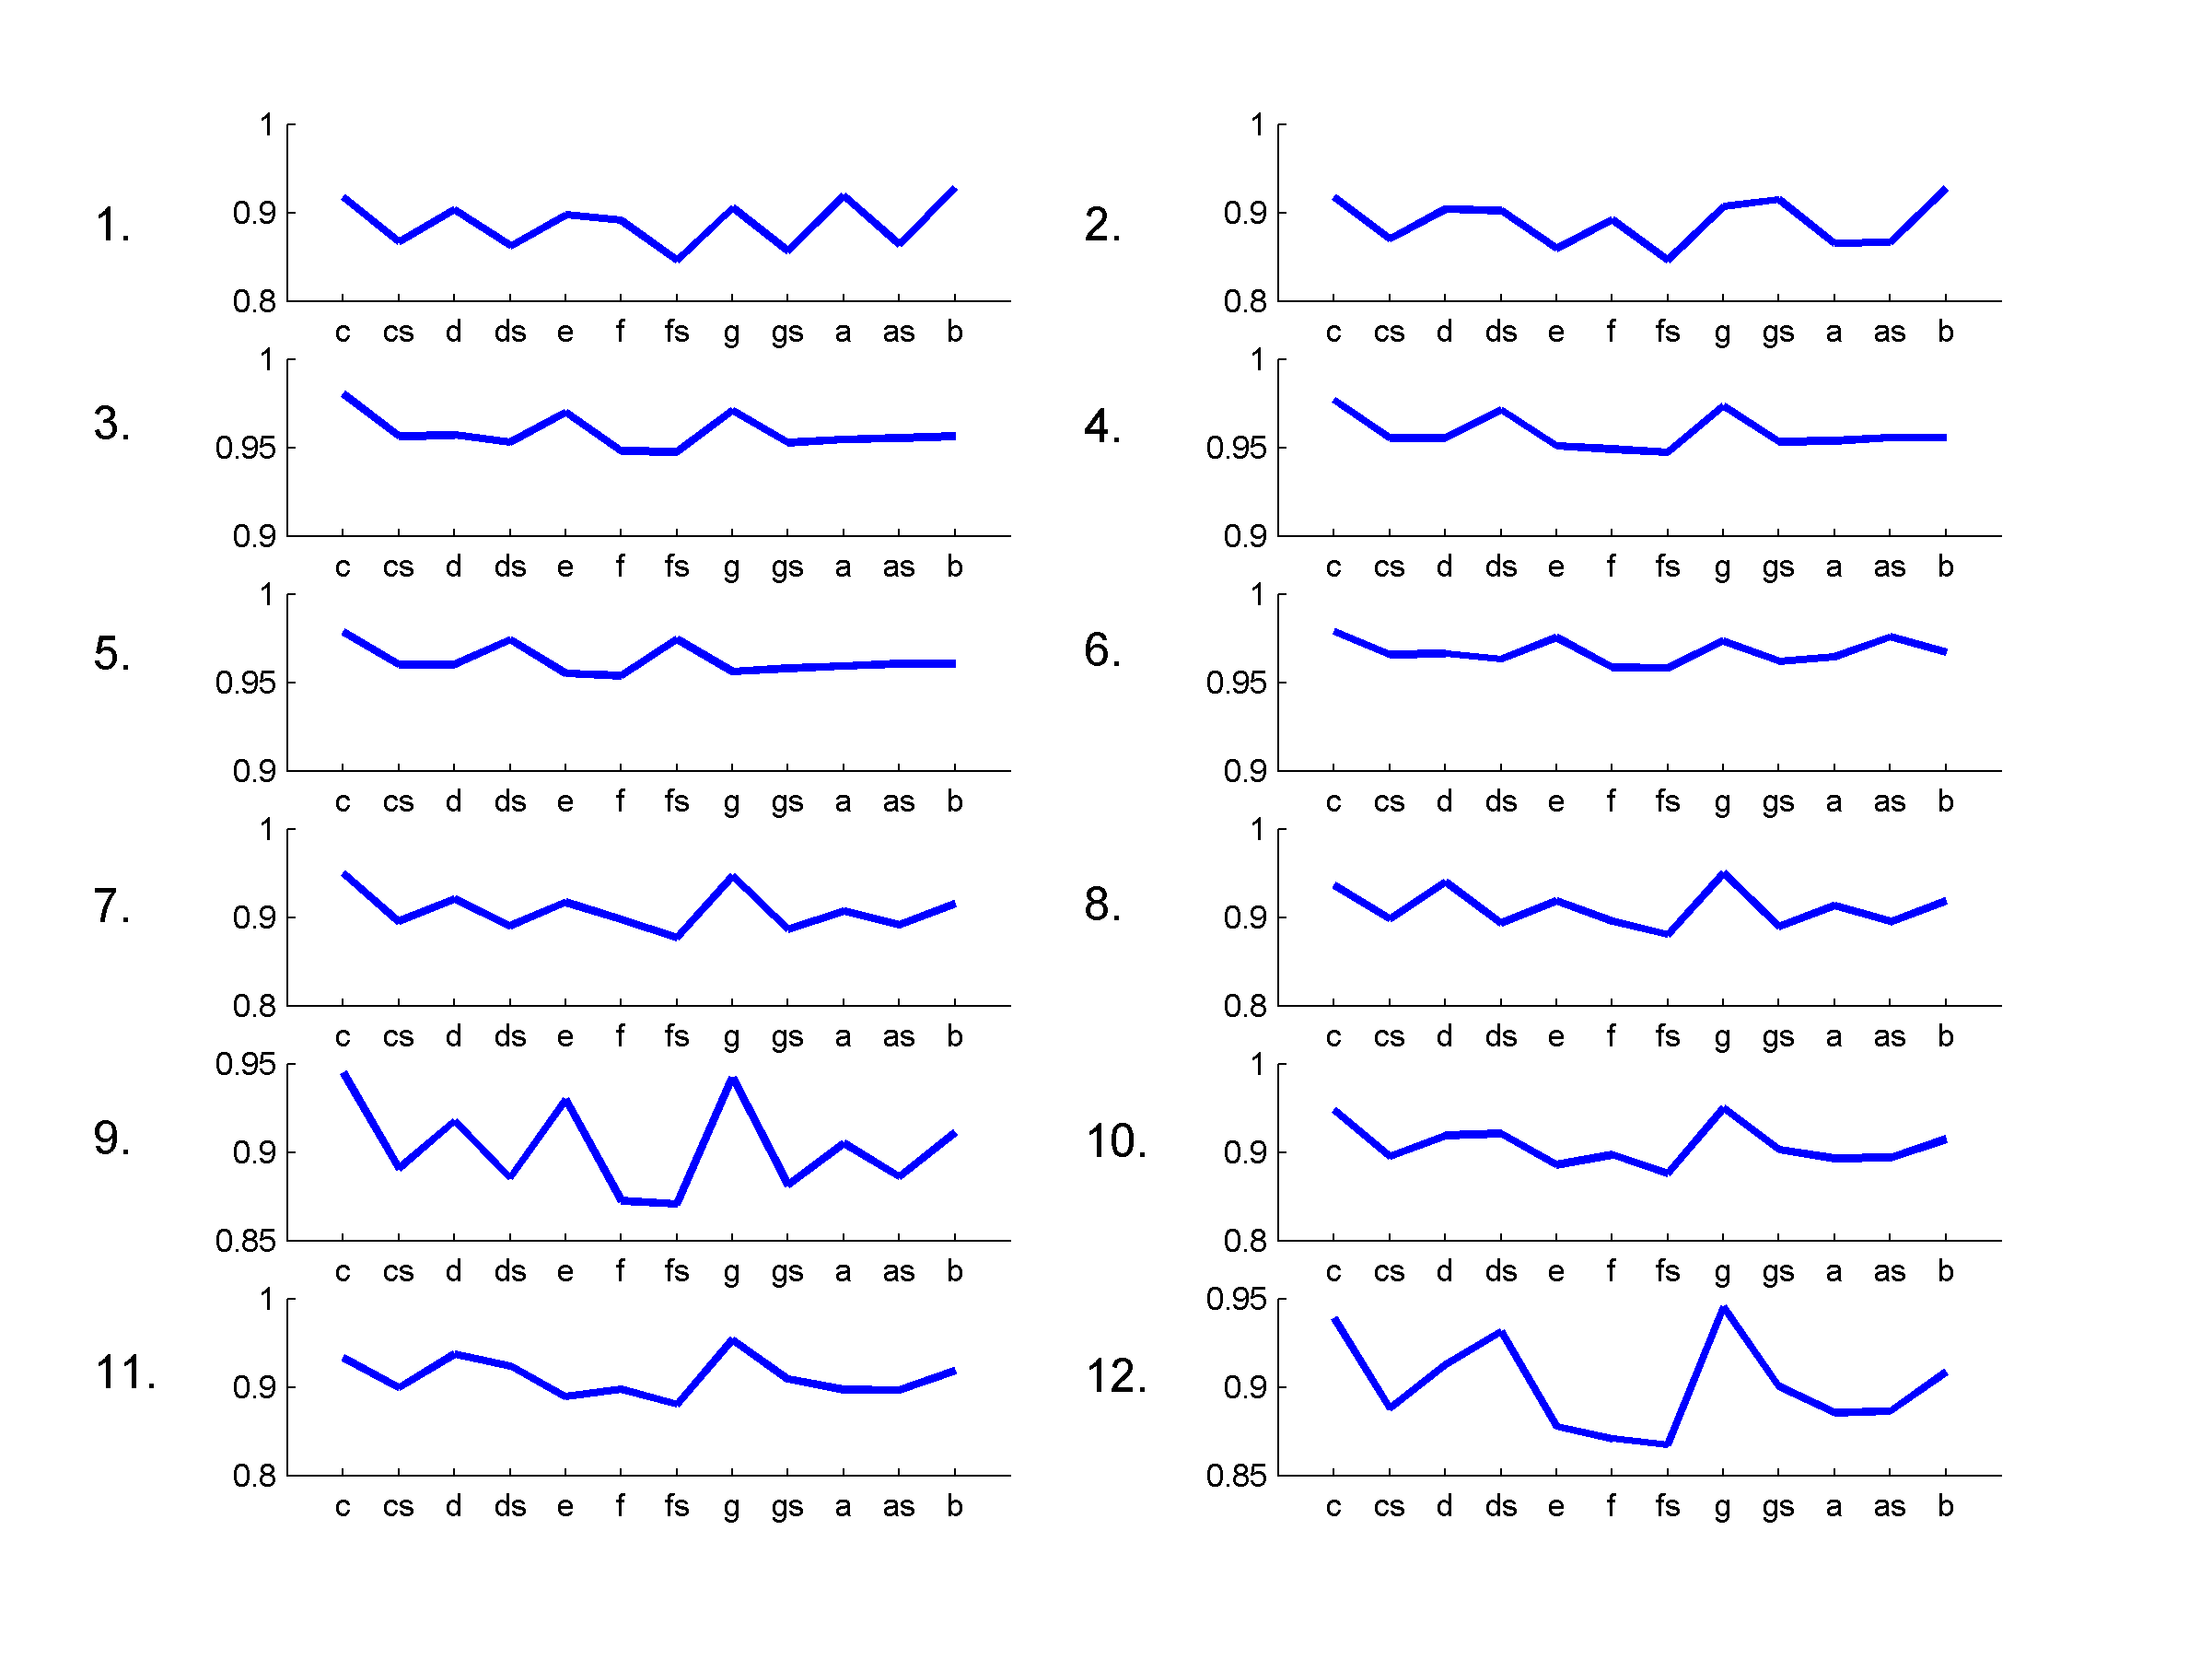
\includegraphics[width=\IPEMDefaultFigureWidth]{Graphics/TonalityDemoFig8}
    \caption{Profiles of 12 context-defining sequences for tone center $T=1.5$.}
    \label{Fig:TonalityDemoFig8}
\end{figure}

For each figure, the vertical axis represents the correlation
between the local image and the global image at the end of the
trial (12 trials are represented in each figure). What matters is
the relative relationships between the correlation coefficients
within a profile. In fact, when profiles are compared with each
other, using the correlation coefficient as a measure of
comparison, then the relative values are important. Table
\ref{table_two} shows the similarities among the twelve profiles.

\begin{table}[!h]
\footnotesize
\begin{tabular}{l|llllllllllll}
element&1.&2.&3.&4.&5.&6.&7.&8.&9.&10.&11.&12 \\ \hline 1.
&1.000&0.457&0.421&0.219&-0.226&0.336&0.709&0.720&0.665&0.428&0.408&0.315\\
2.
&&1.000&0.208&0.439&-0.024&0.090&0.404&0.384&0.289&0.698&0.708&0.671\\
3.
&&&1.000&0.670&0.163&0.867&0.865&0.724&0.916&0.647&0.492&0.589\\
4. &&&&1.000&0.466&0.531&0.647&0.525&0.588&0.887&0.756&0.923\\ 5.
&&&&&1.000&0.053&0.000&-0.140&0.010&0.224&0.065&0.332\\ 6.
&&&&&&1.000&0.677&0.577&0.770&0.457&0.334&0.435\\ 7.
&&&&&&&1.000&0.938&0.940&0.794&0.712&0.659\\ 8.
&&&&&&&&1.000&0.910&0.727&0.768&0.629\\ 9.
&&&&&&&&&1.000&0.662&0.609&0.611\\ 10.
&&&&&&&&&&1.000&0.936&0.943\\ 11. &&&&&&&&&&&1.000&0.917\\ 12.
&&&&&&&&&&&&1.000\\
\end{tabular}
\caption{The correlation coefficients represent the similarity
between the profiles, for the 12 context-defining sequences used
in Simulation I}
\label{table_two}
\end{table}
%
The following observations can be made:
\begin{itemize}
\item
Sequence 1 (major scale) correlates best with sequences 7, 8, and
9 (the cadences in major). The average correlation between the
major scale (1) and the three cadences in major (7, 8, 9) is
0.698. It was 0.796 in the data of Krumhansl and Kessler.
\item
Sequence 2 (minor scale) correlates best with sequences 10, 11, 12
(the cadences in minor). The average correlation between the minor
scale (2) and the three cadences in minor (10, 11, 12) is 0.6923.
It was 0.727 in the data of Krumhansl and Kessler
\item
Sequence 3 (major chord) correlates best with sequences 6, 7, 8,
and 9 (dominant seventh chord and major cadences). The average
correlation between the major chord (3) and the three cadences in
major (7, 8, 9) is 0.835. It was 0.896 in the data of Krumhansl
and Kessler.
\item
Sequence 4 (minor chord) correlates best with sequences 10, 11, 12
(minor cadences). The average correlation between the minor chord
(4) and the three cadences in minor (10, 11, 12) is  0.855. It was
0.910 in the data of Krumhansl and Kessler.
\item
Sequence 5 (diminished chord) has a low correlation with all other
sequences.
\item
Sequence 6 (dominant seventh chord) has the highest correlation
with sequence 9 (VI V I cadence in major).
\item
All cadences in major are strongly connected, and all cadences in
minor are strongly connected.
\end{itemize}

Krumhansl and Kessler concluded that the major chord element and
the three cadences in major indicate a consistent pattern of
ratings. In a similar way, the major scale was somewhat less
similar. They therefore took the major key profile as the average
ratings, given the 12 probe tones, for the major chord and the
three cadences in major. In correspondence with this idea, and
justified by the results shown in Table \ref{table_two}, the major
key profile of Simulation I is defined as the average of the
profiles that correspond to the sequences 3, 7, 8, and 9. The
minor key profile of Simulation I is determined according to the
same reasoning, taking the average of the profiles that correspond
to the sequences 4, 10, 11, and 12. The similarity of the major
key profile of Experiment I with the major key profile of
Simulation I has correlation coefficient of 0.848. The similarity
of the minor key profile of Experiment I with the minor key
profile of Simulation I is 0.825. This is a significant
correlation showing that the short-term memory model gives a good
account of the data in Experiment I.\\ An important parameter of
the model pertains to the echo of the global images. In order to
clarify the role of the echo, a series of simulations are carried
out in which the echo of the global image is systematically
varied from $T=0.2$ to $T=5$ in steps of 0.2. Twenty-five figures
are plotted that show the effect of changing the echo $(T)$ of the
global images on the profiles of the 12 context-defining
sequences. Each time the 144 trials are processed. Figures
\ref{Fig:TonalityDemoKK1Fig2} to \ref{Fig:TonalityDemoKK1Fig17} show the 12 profiles for
halfdecay tone centers with the echo set to $T=0.4$, $T=1.4$, $T=2.4$ and $T=3.4$\\

\begin{figure}[p]
    \centering
    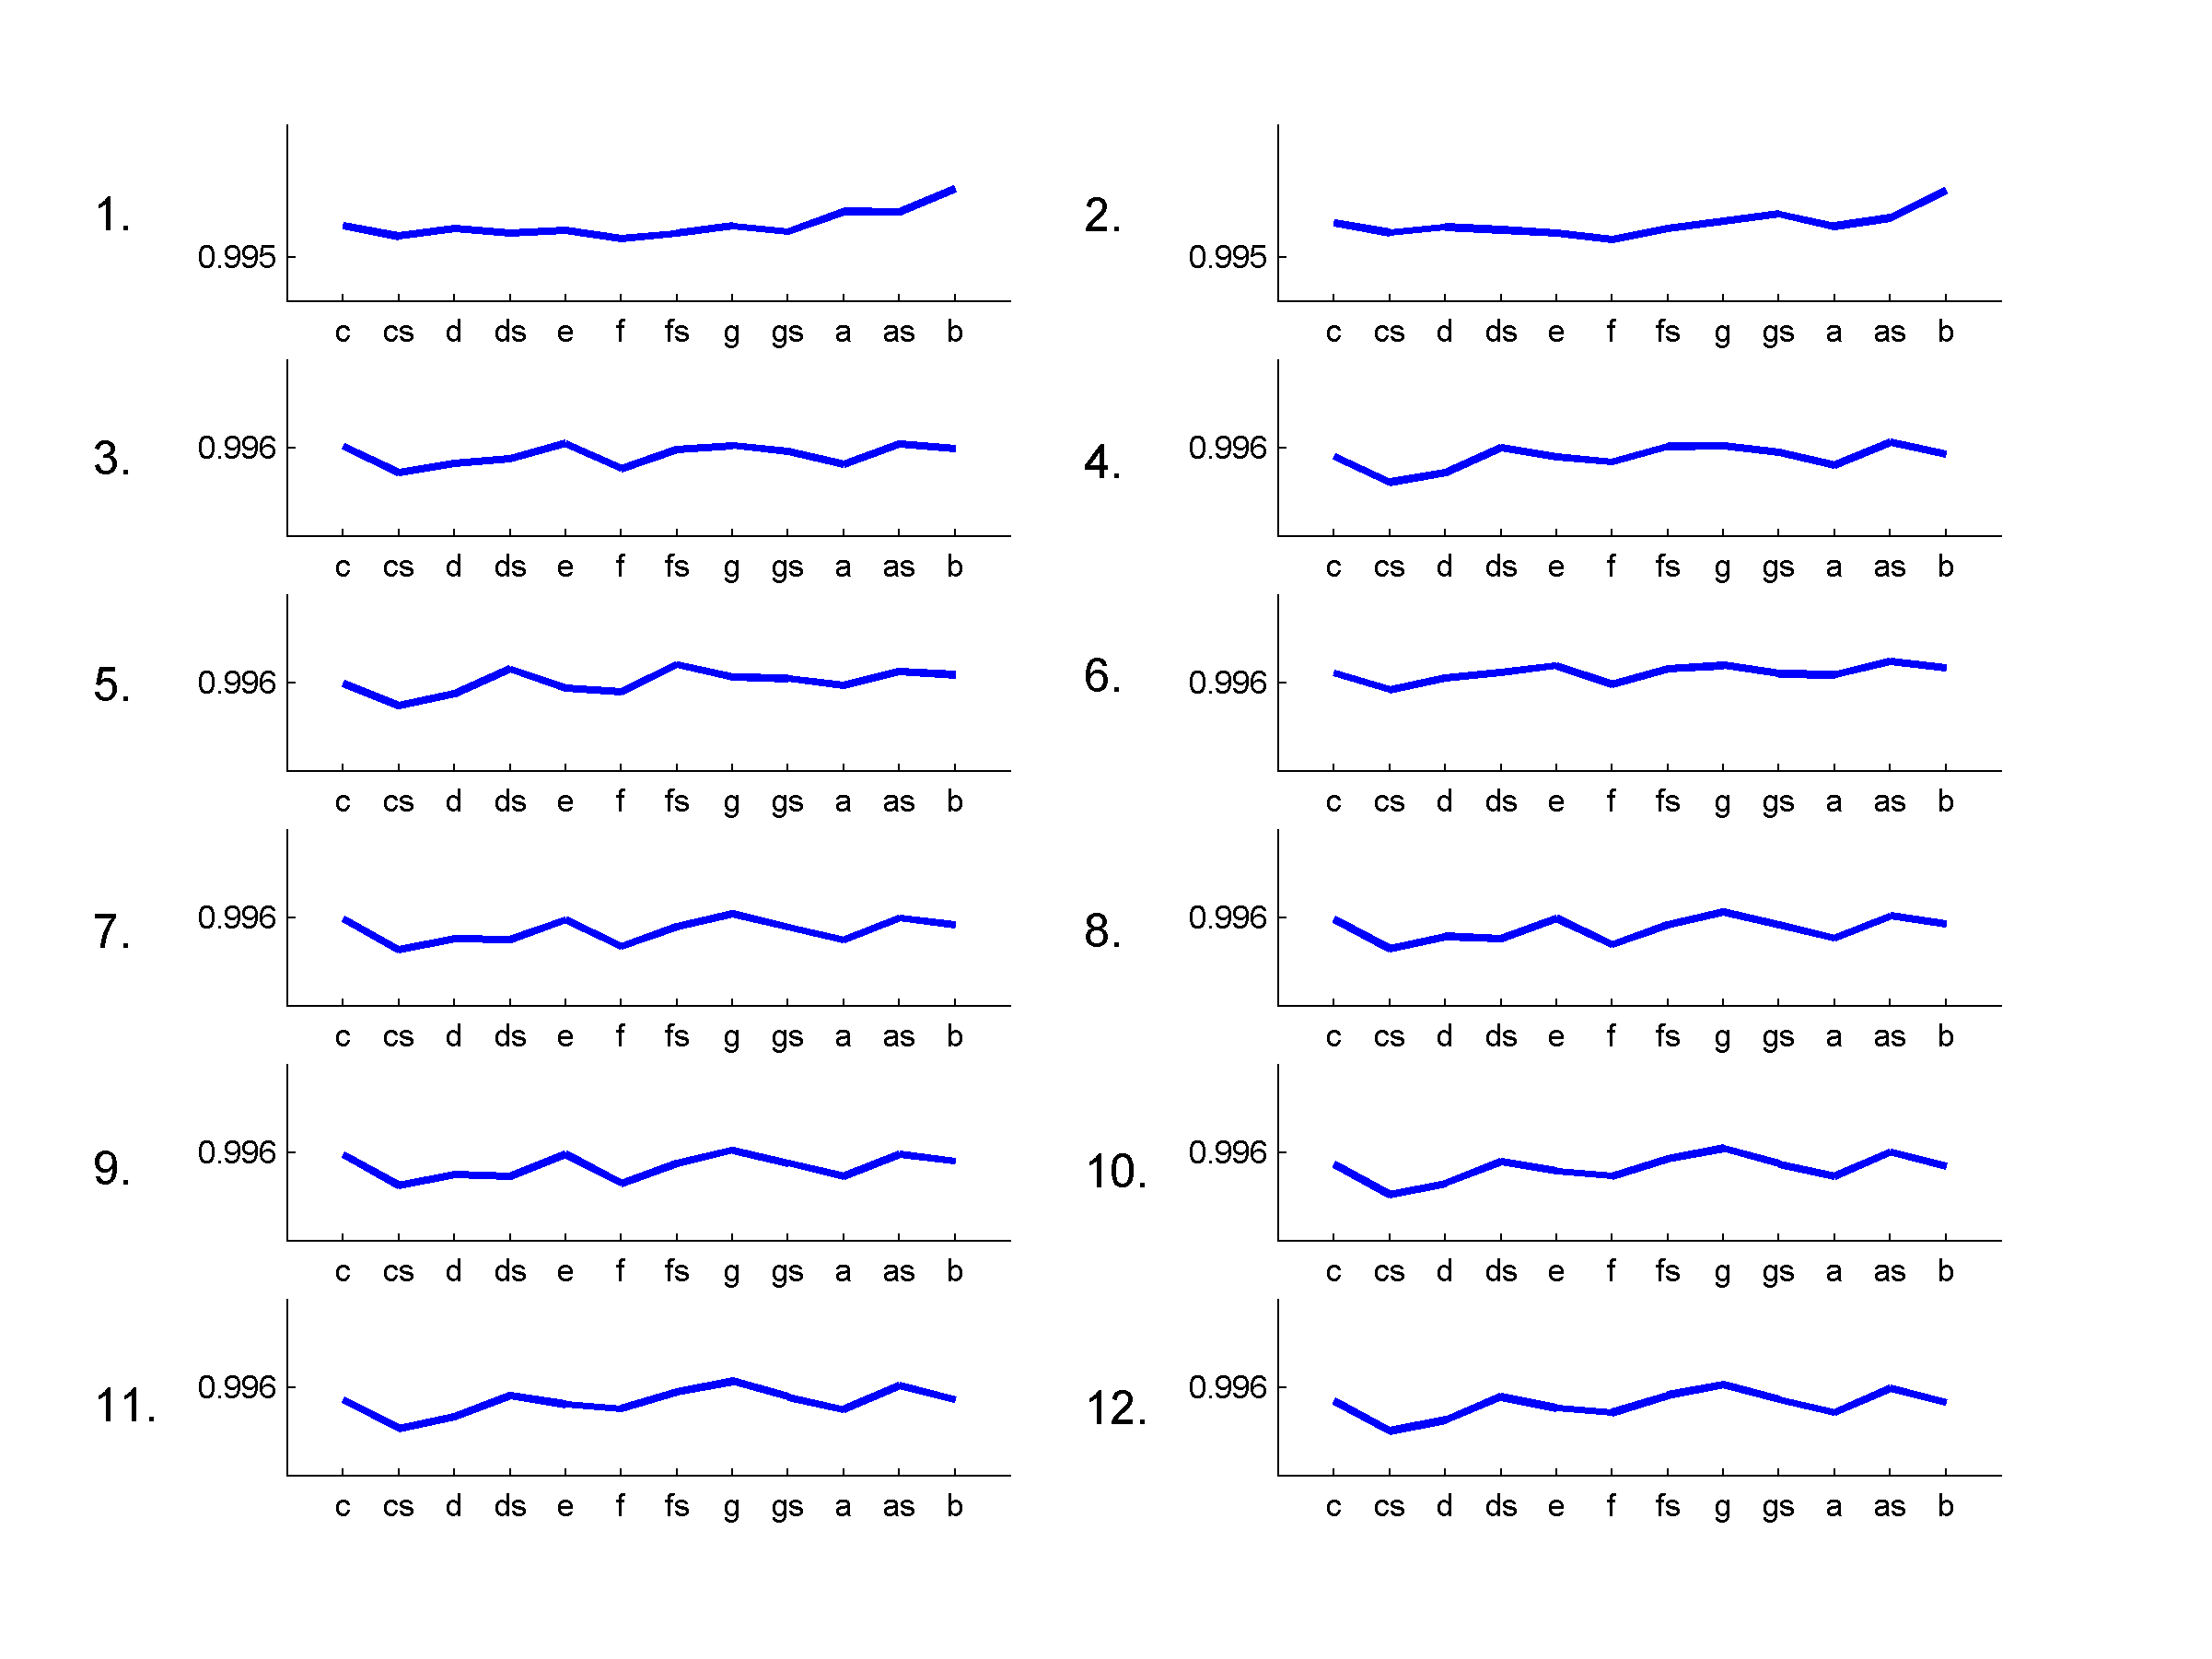
\includegraphics[width=\IPEMDefaultFigureWidth]{Graphics/TonalityDemoKK1Fig2}
    \caption{Profiles of 12 context-defining sequences for tone center $T=0.4.$}
    \label{Fig:TonalityDemoKK1Fig2}
\end{figure}

\begin{figure}[p]
    \centering
    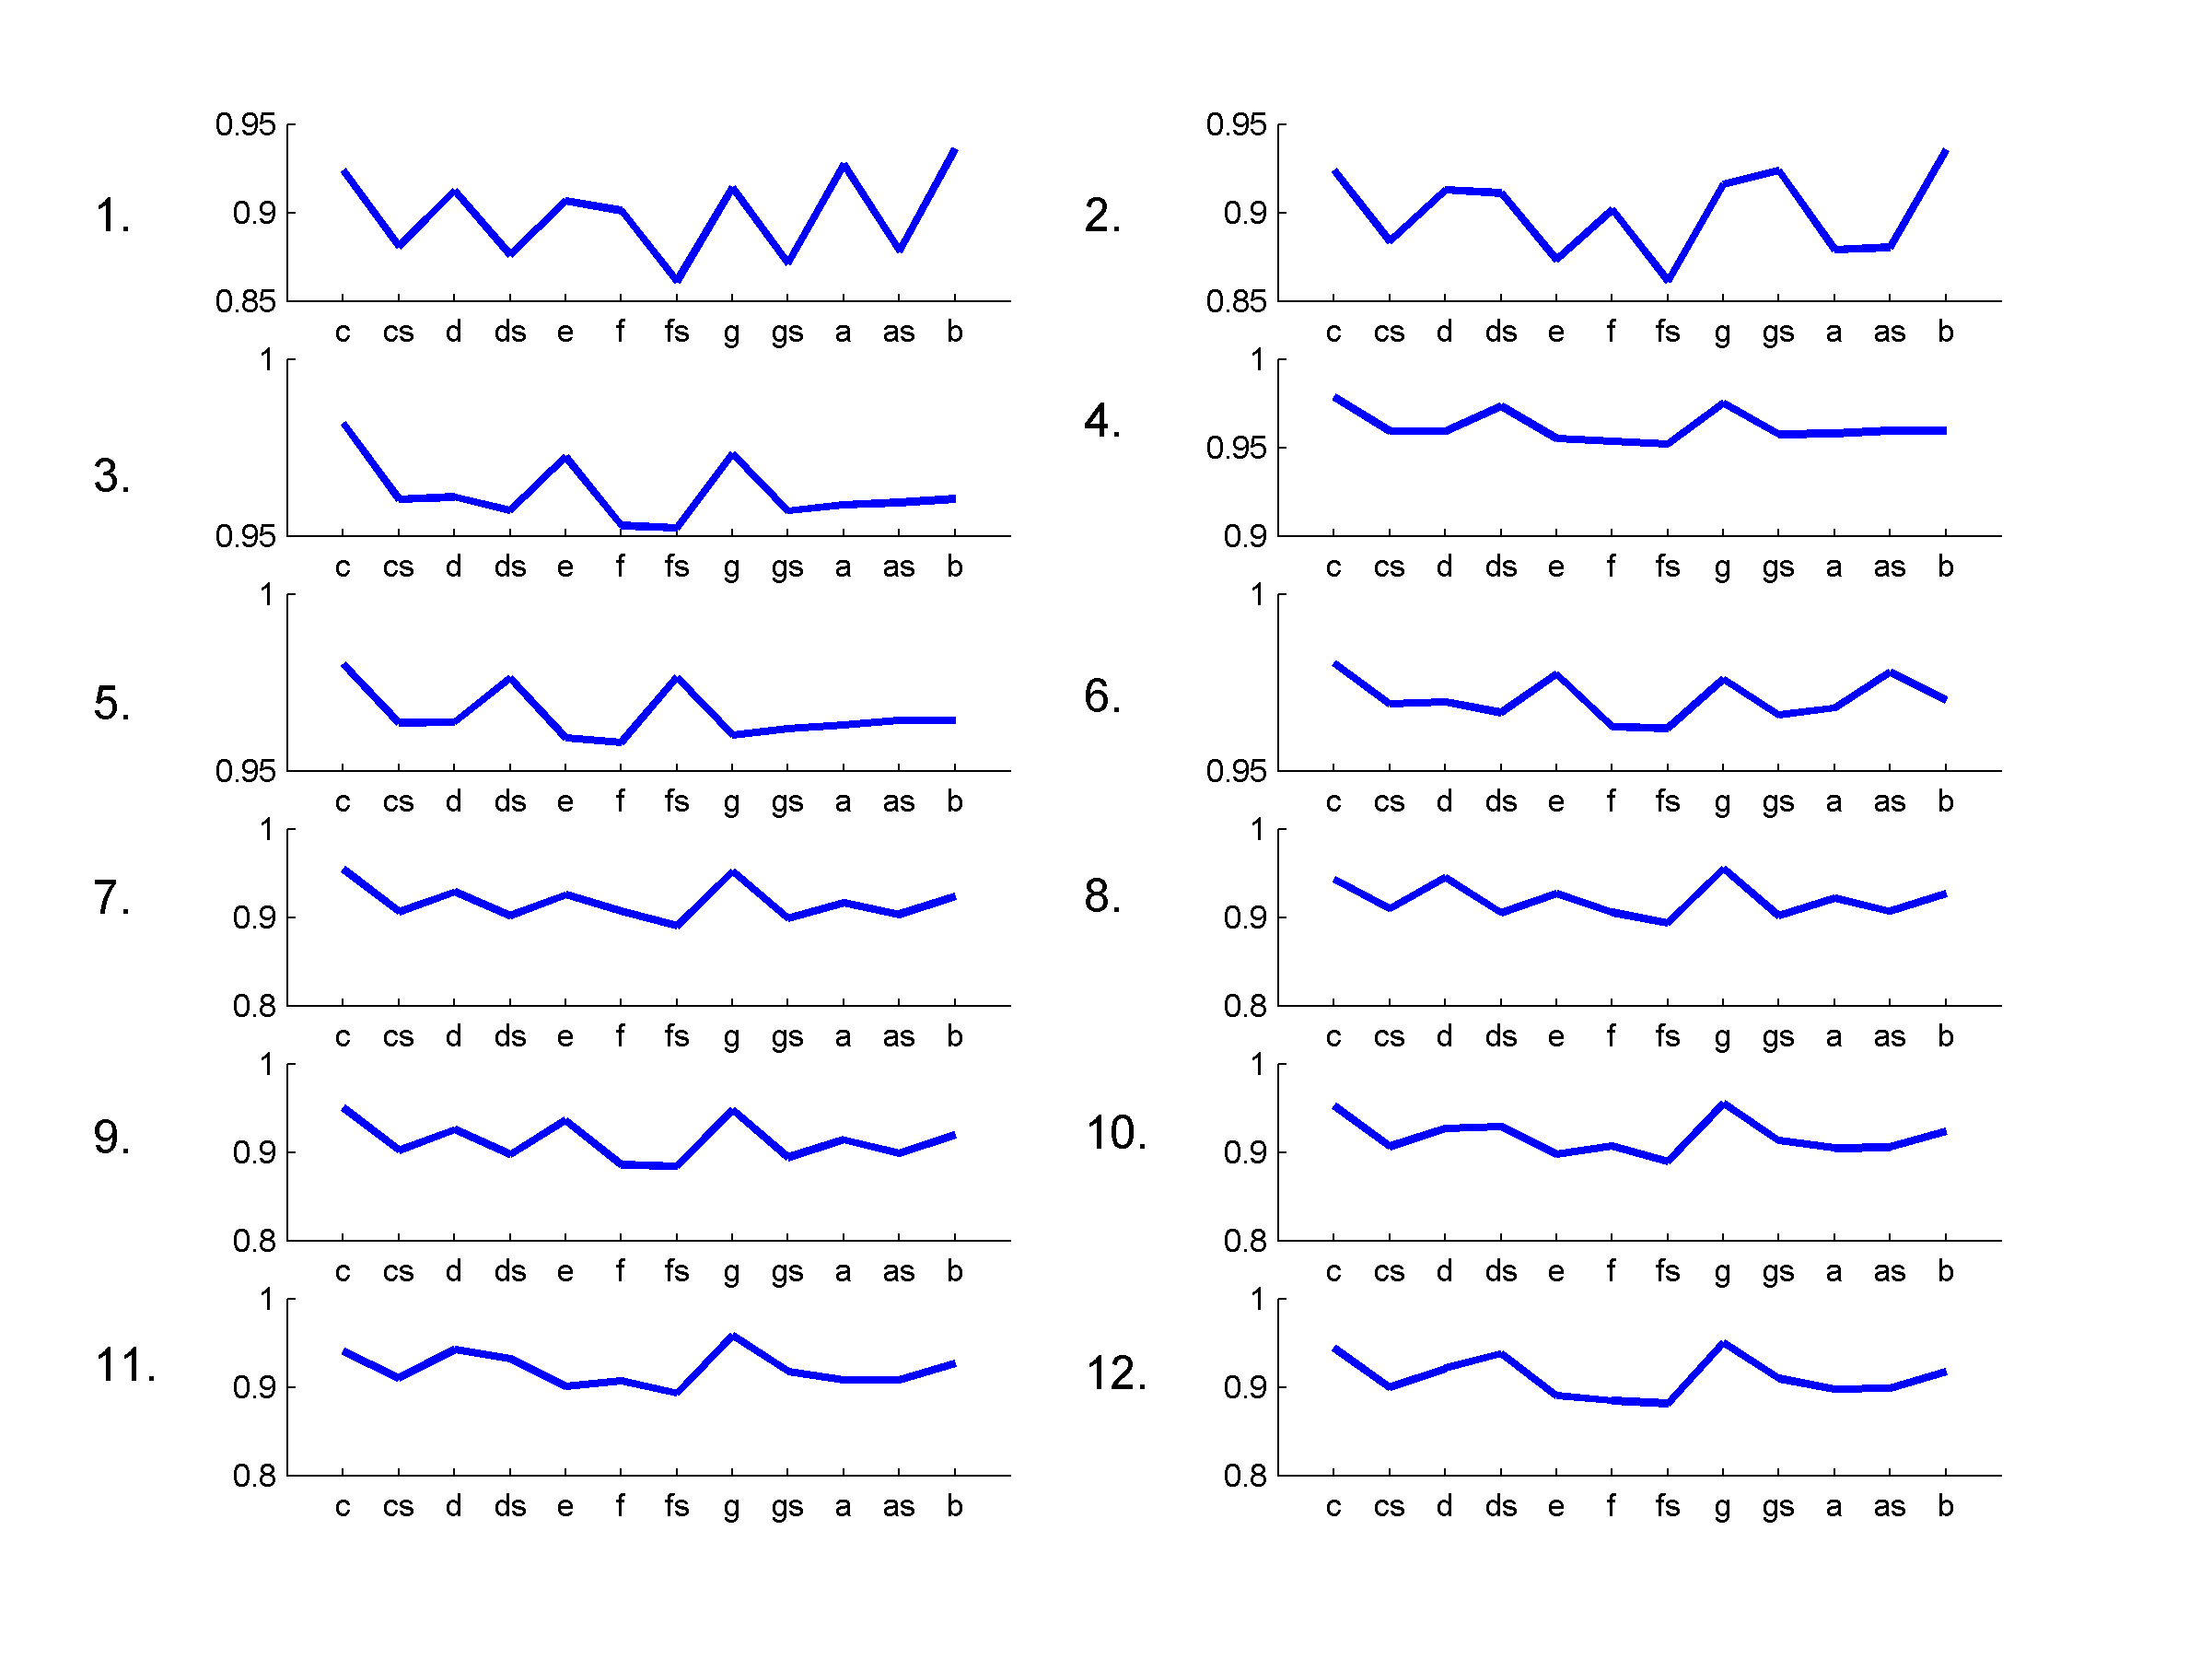
\includegraphics[width=\IPEMDefaultFigureWidth]{Graphics/TonalityDemoKK1Fig7}
    \caption{Profiles of 12 context-defining sequences for tone center $T=1.4.$}
    \label{Fig:TonalityDemoKK1Fig7}
\end{figure}

\begin{figure}[p]
    \centering
    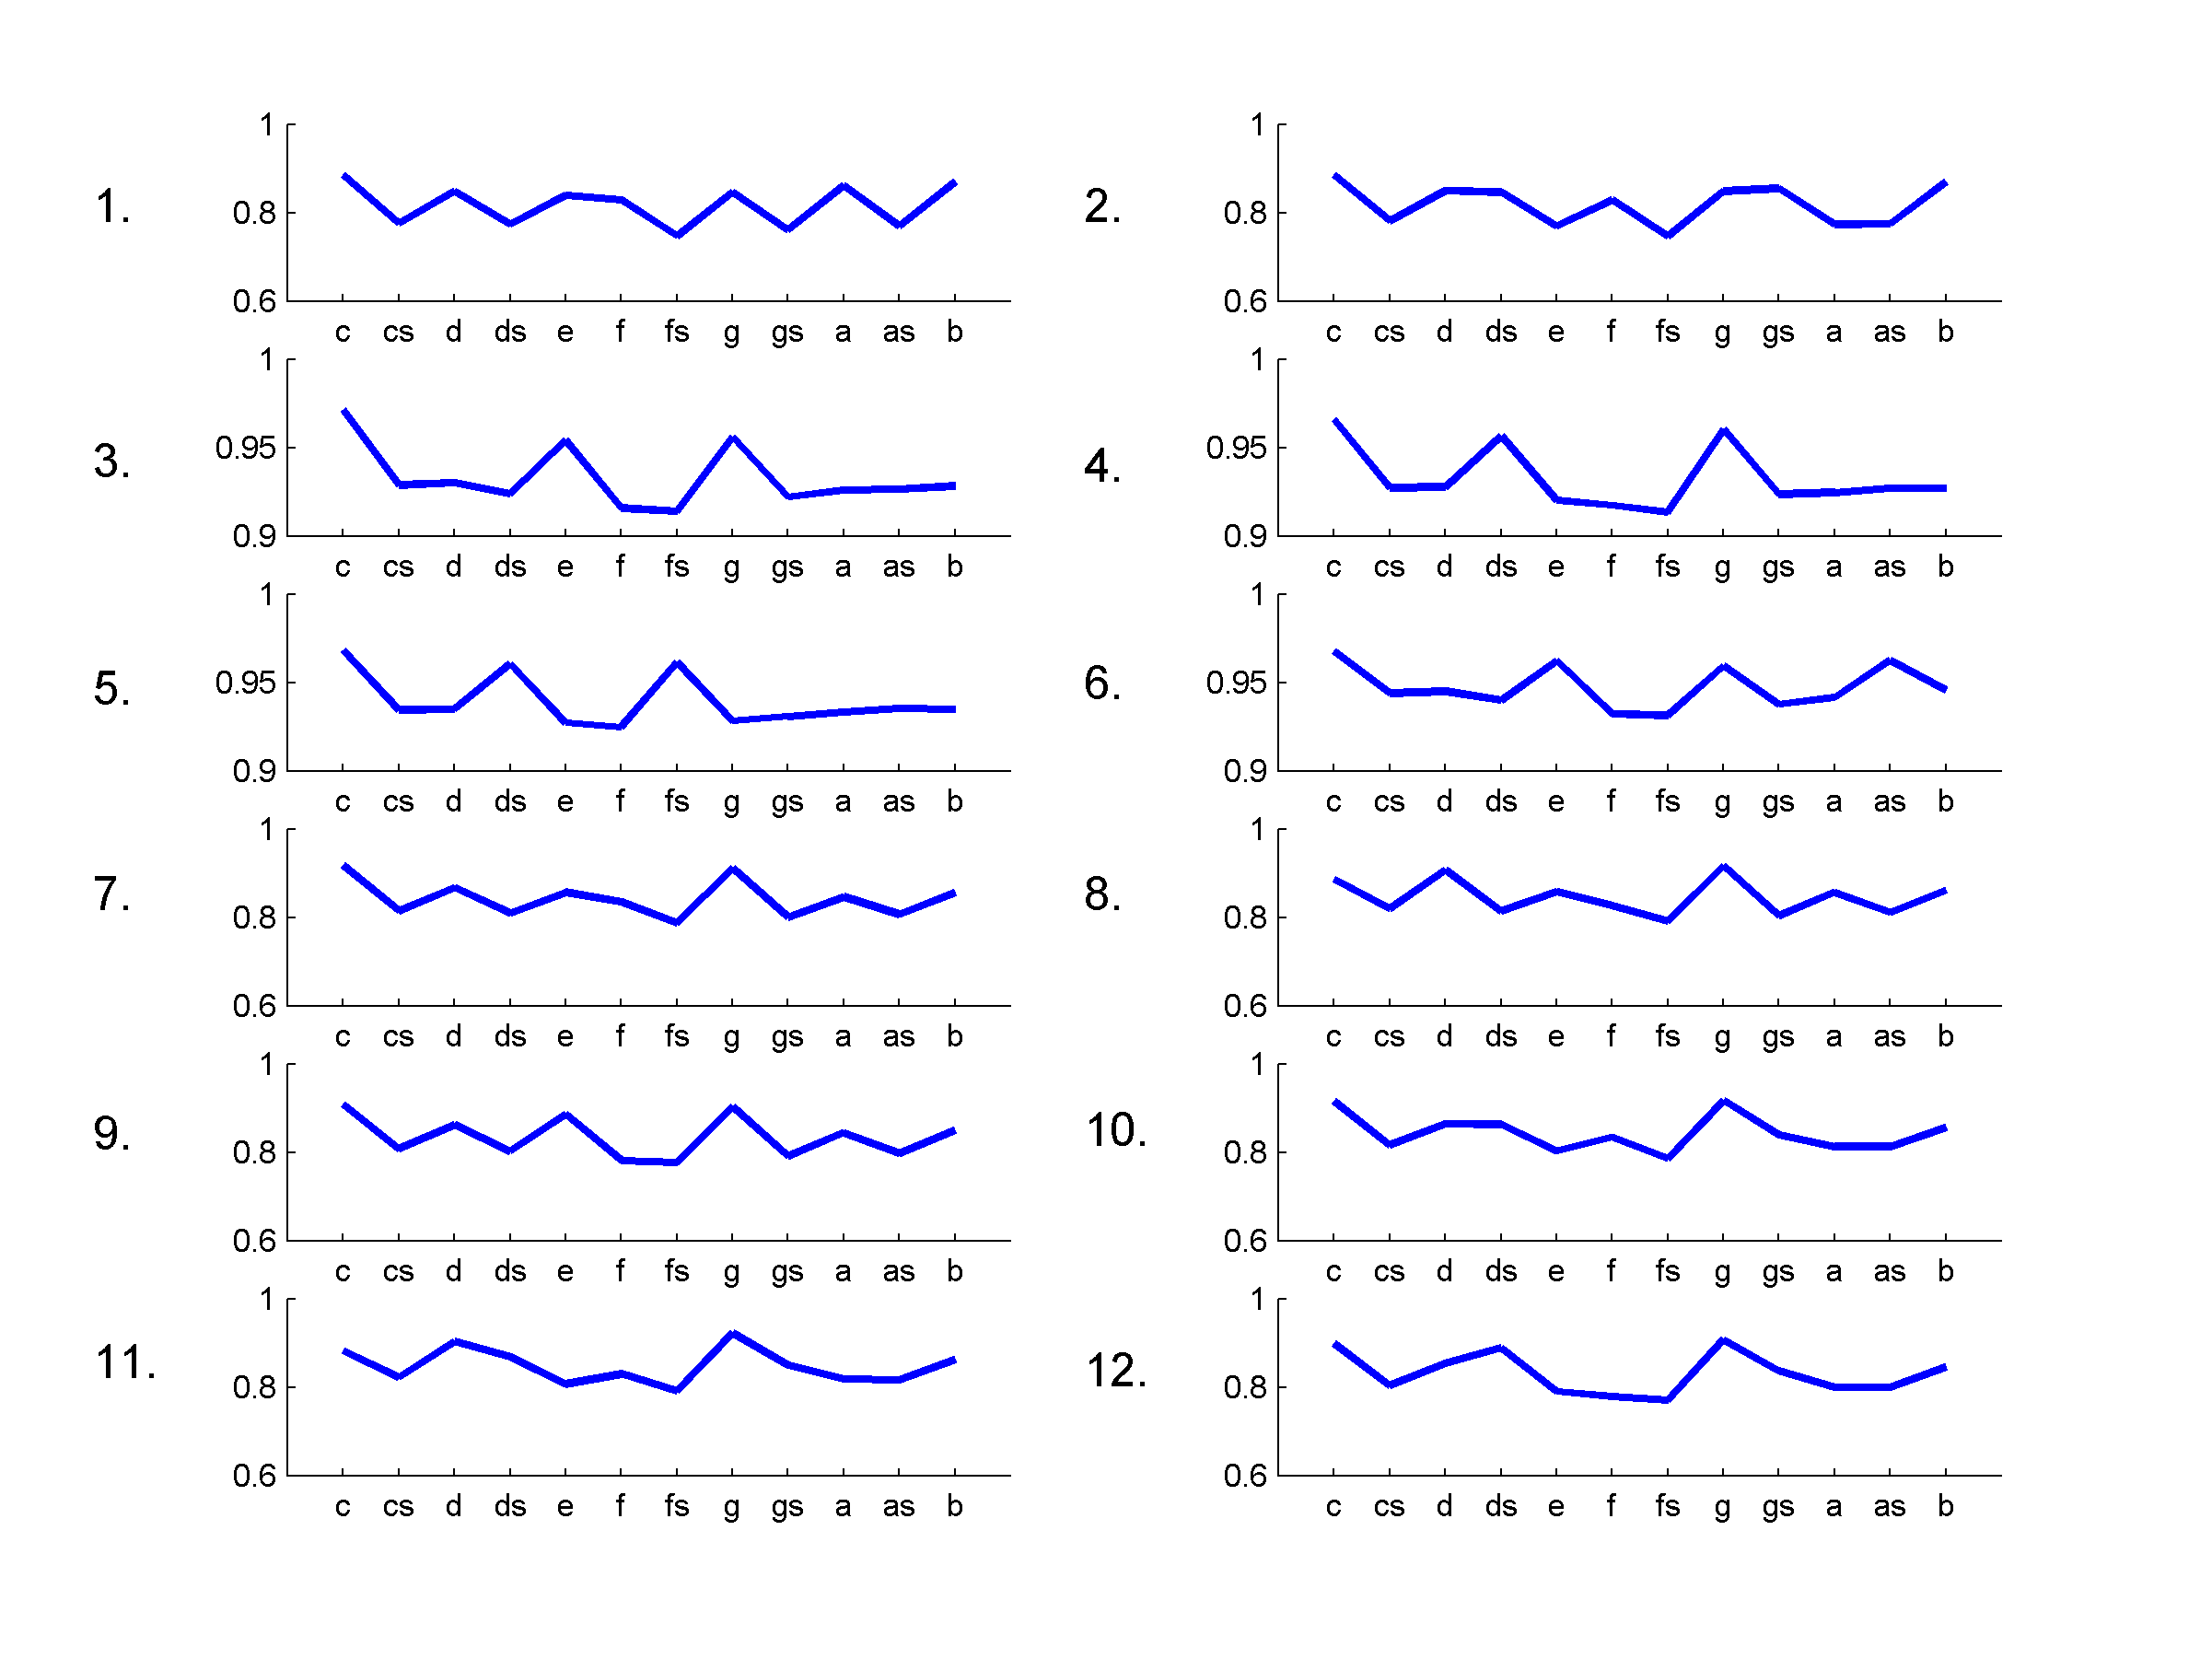
\includegraphics[width=\IPEMDefaultFigureWidth]{Graphics/TonalityDemoKK1Fig12}
    \caption{Profiles of 12 context-defining sequences for tone center $T=2.4.$}
    \label{Fig:TonalityDemoKK1Fig12}
\end{figure}

\begin{figure}[p]
    \centering
    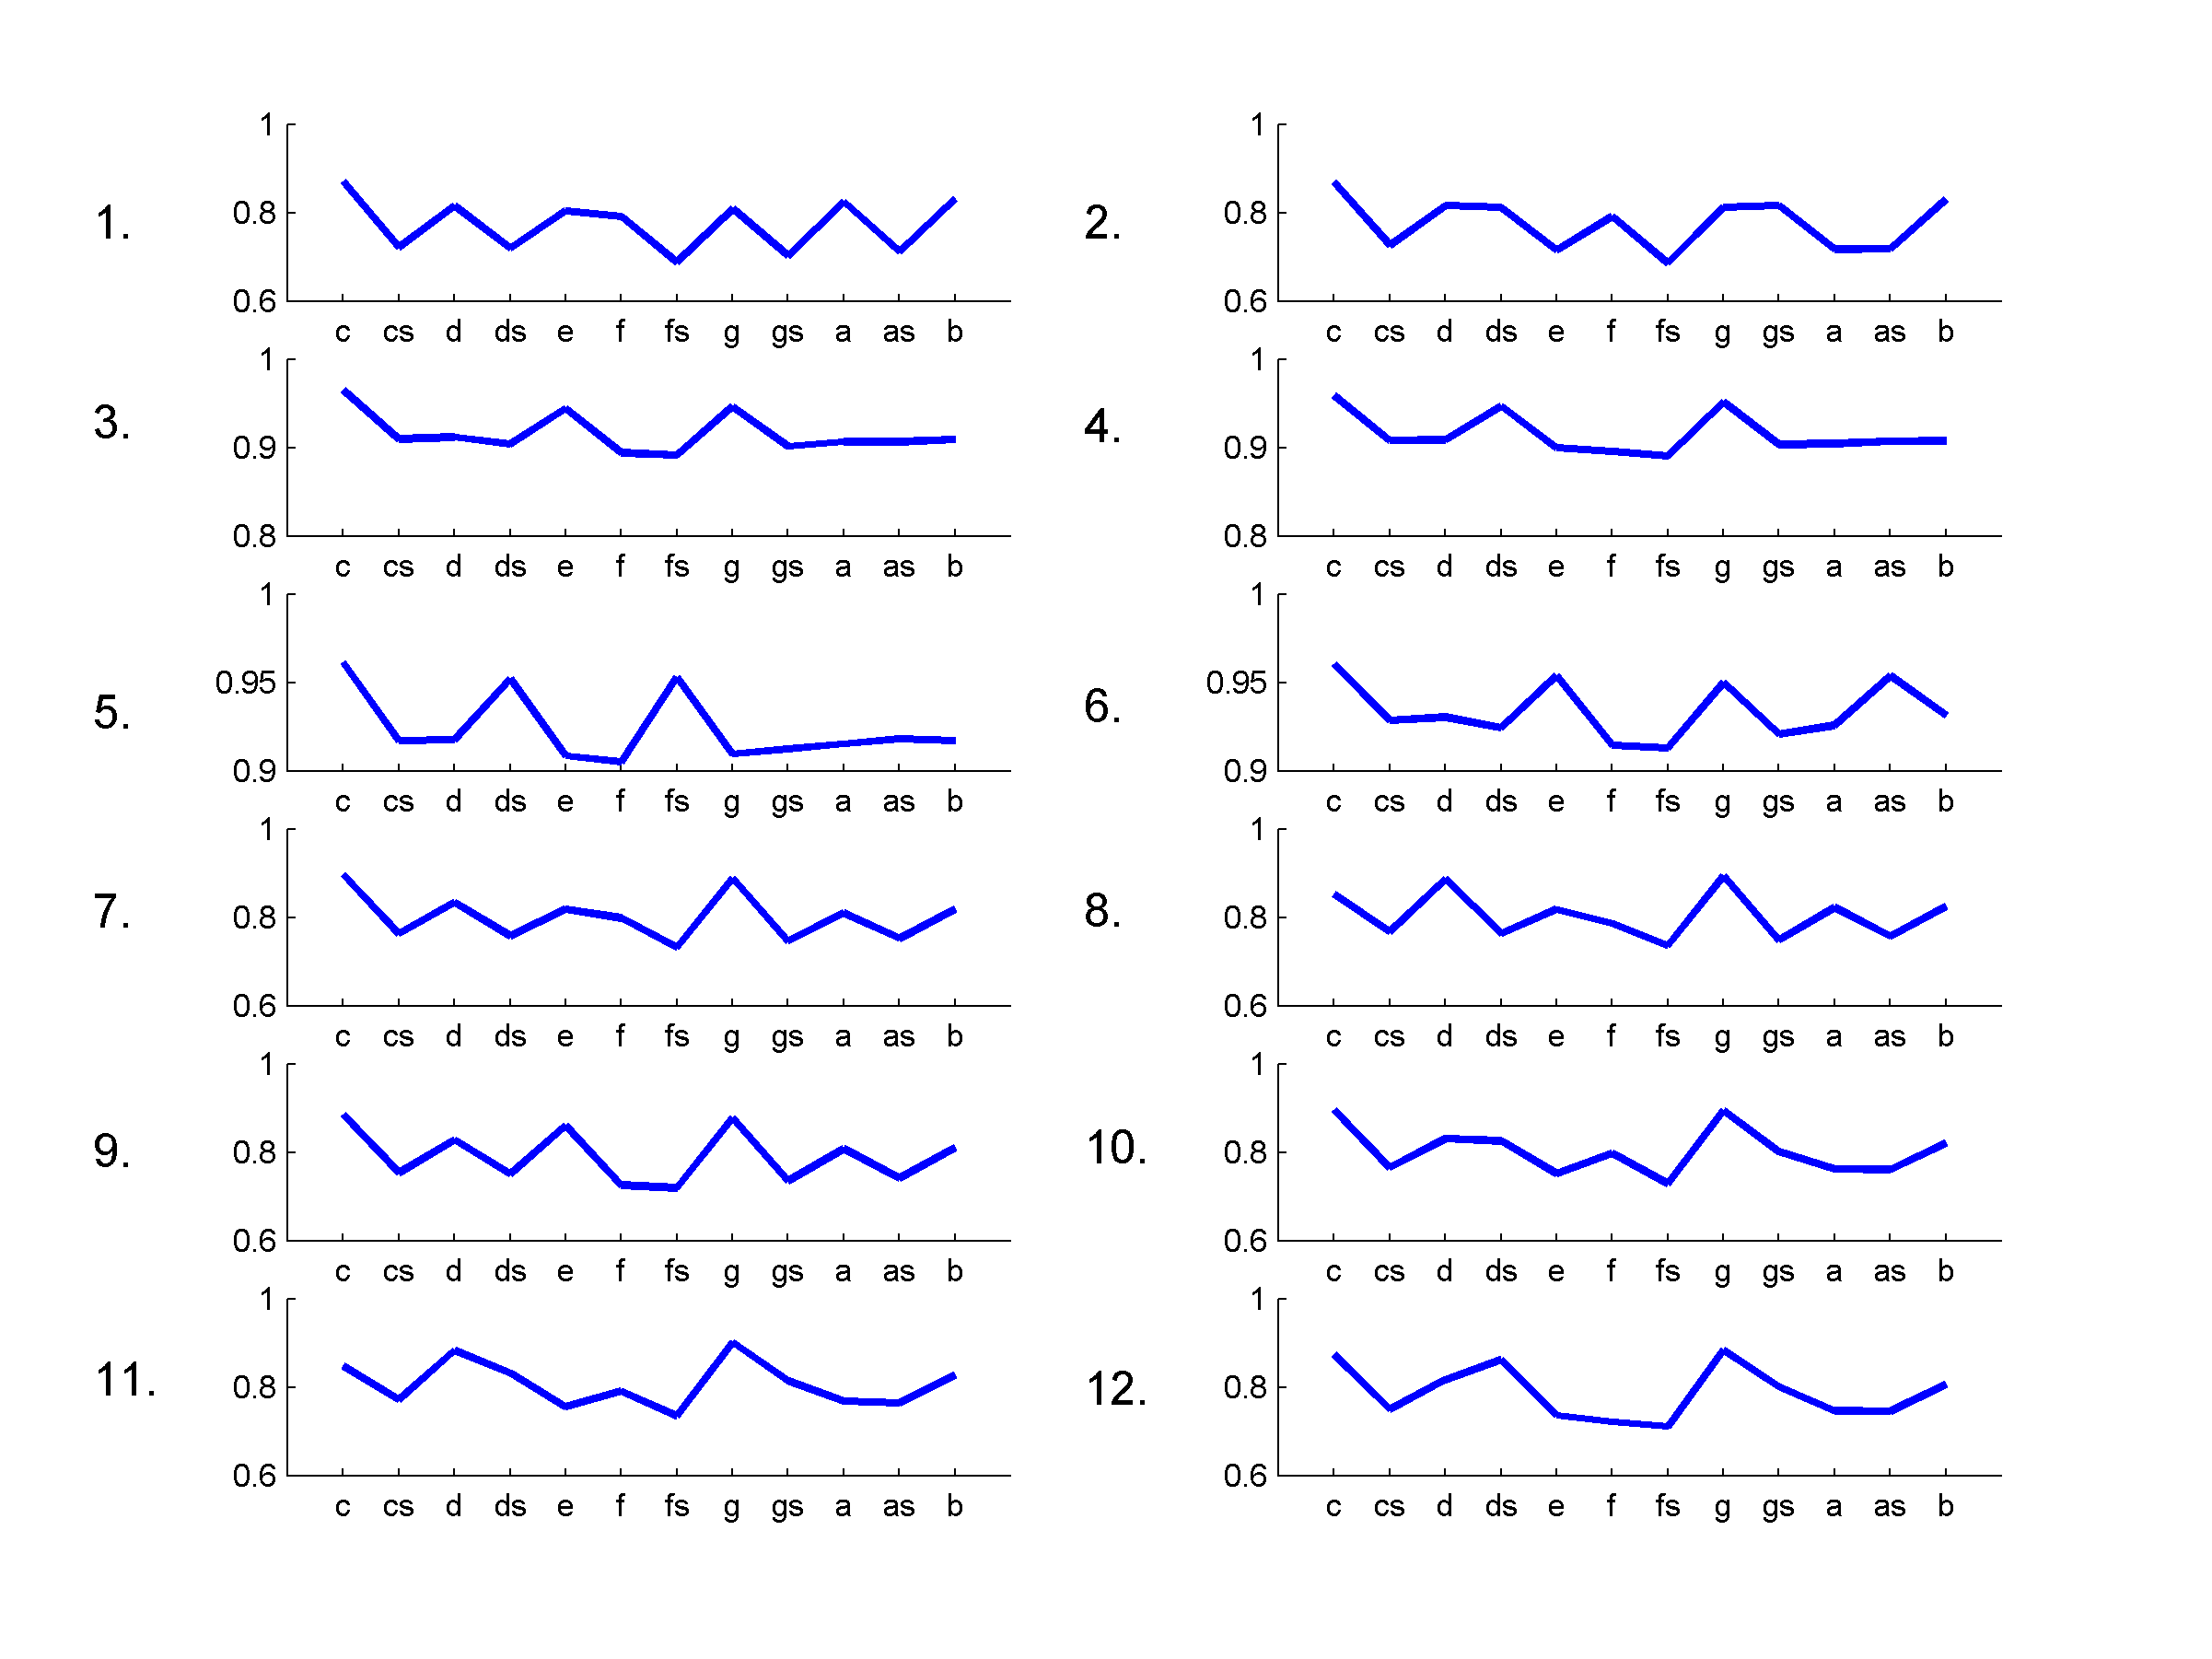
\includegraphics[width=\IPEMDefaultFigureWidth]{Graphics/TonalityDemoKK1Fig17}
    \caption{Profiles of 12 context-defining sequences for tone center $T=3.4.$}
    \label{Fig:TonalityDemoKK1Fig17}
\end{figure}

\subsubsection* {Simulation II}
% --------------------------------------------------------------------------------

Simulation II corresponds to Experiment II that aimed at sensing
directly how the listener's sense of key develops and changes,
providing a quantitative measure of the relative strengths of
tonal interpretations at each point in time. The test uses 10
different chord sequences containing modulations from one key to
another key. Table \ref{ChordSequences} gives an overview of the
10 different chord sequences. The sequences, ordered from 1 to 10
are each composed of 9 chords. They have a starting key and an
ending key, and the modulation from one key to the other key can
be direct, indirect, close, or remote.\\
Sequence 1 has no modulation, starting and ending key are in C
major.\\
Sequence 2 has no modulation, starting and ending key are in C
minor.\\
Sequence 3 has a direct and close modulation, starting in C major
and ending in G major.\\
Sequence 4 has an indirect and remote modulation, starting in C
major and ending in B$\flat$ major.\\
Sequence 5 has a direct and close modulation, starting in C major
and ending in A minor.\\
Sequence 6 has an indirect and remote modulation, starting in C
major and ending in D minor.\\
Sequence 7 has a close modulation, starting in C minor and ending
in F minor.\\
Sequence 8 has a remote modulation, starting in C minor and
ending in C$\sharp$ minor.\\
Sequence 9 has a close modulation, starting in C minor and ending
in C major.\\
Sequence 10 has an indirect and close modulation, starting in C
minor and ending in A$\flat$ major.\\
\begin{table} [!h]
    \footnotesize
    \centering
    \small Chords\\ \vspace{1cm}
    \begin{tabular}{l|lllllllll}
        % after \\ : \hline or \cline{col1-col2} \cline{col3-col4} ...
        & 1 & 2 & 3 &4 & 5 & 6 & 7 & 8 & 9 \\ \\\hline\\
        Seq.~1: & Fmaj & Gmaj & Amin        & Fmaj & Cmaj & Amin  & Dmin   & Gmaj &
        Cmaj\\\\
        Seq.~2: & Fmin & Gmaj & A$\flat$maj & Fmin & Cmin & A$\flat$maj & Ddim & Gmaj & Cmin \\\\
        Seq.~3: & Fmaj & Gmaj & Cmaj & Amin & Emin & Bmin & Emin & Dmaj & Gmaj \\\\
        Seq.~4: & Fmaj & Gmaj & Cmaj & Amin & Fmaj & Gmin & E$\flat$maj & Fmaj & B$\flat$maj \\\\
        Seq.~5: & Fmaj & Gmaj & Cmaj & Fmaj & Dmin & Emaj & Bdim & Emaj & Amin \\\\
        Seq.~6: & Fmaj & Gmaj & Cmaj & Fmaj & Dmin & B$\flat$maj & Edim & Amaj & Dmin \\\\
        Seq.~7: & Ddim & Gmaj & Cmin & A$\flat$maj & Fmin & D$\flat$maj & B$\flat$min &
        Cmaj & Fmin \\\\
        Seq.~8: & Ddim & Gmaj & Cmin & Gmaj & A$\flat$maj & Amaj & F$\sharp$min &
        G$\sharp$maj & C$\sharp$min \\\\
        Seq.~9: & Ddim & Gmaj & Cmin & A$\flat$maj & Gmaj & Amin & Fmaj & Gmaj & Cmaj \\\\
        Seq.~10: & Ddim & Gmaj & Cmin & A$\flat$maj & Fmin & E$\flat$maj & B$\flat$min &
        E$\flat$maj & A$\flat$maj \\\\
    \end{tabular}
    \caption{\ Chord Sequences Used in Experiment II.
    Cmaj means the C major chord, Cmin the C minor chord, and Cdim,
    the C diminished chord.}
    \label{ChordSequences}
\end{table}

A single chord sequence consists of 9 chords and for each
sequence, there were 9 trials. In the first trial, the
context-defining sequence was limited to the first chord and the
listeners were asked to probe the chord with the 12 probe tones.
In the second trial, the context-defining sequence was made of the
first two chords of the sequence and the listeners were asked to
probe this two-chord sequence with the 12 probe tones. In the
third trial, the context-defining sequence was made of the first
three chords of the sequence and the listeners were asked to probe
the sequence with the 12 probe tones, and so on. In the ninth
trial, the context-defining sequence was equal to the complete
sequence. For each chord sequence, one thus obtained 9 profiles
containing information about the gradual temporal deployment of
the tonal sequence. The 10 different chord sequences thus
correspond to 10 different {\sl profile-sequences}, each
containing 9 profiles.\\\\

The analysis of a profile-sequence had two parts. In the first
part the analysis was done in reference to the profile of the
first key of the corresponding chord sequence. In the second part,
the analysis was done in reference to the second key of the
corresponding chord sequence. Thus, if the chord sequence started
in C major, and modulated to G major, then the first analysis
correlated each profile of the sequence with the profile of the C
major key. The second analysis correlated each profile of the
sequence with the profile of the G major key. One thus obtained
for each chord sequence two (nine-step) {\sl
correlation-sequences}, one correlation-sequence representing the
sense of key with respect to the first key, another
correlation-sequence representing the sense of key with respect to
the second key.\\\\

Simulation II has then been set up as follows. The 10 chord
sequences with 9 subsequences each, define 90 context-defining
sequences. Each sequence was processed as follows:
\begin{enumerate}
\item
    The sound $s(t)$ of the chord sequence is processed with the
    auditory model (APM, PCM, and EMM) into local and global images.
    The echos are set to $T=0.1$ and $T=1.5$.
\item
    The global images $\tilde{p}_{T=1.5}(t)$ are inspected by the 12
    different probes tones using the stimulus-driven inference Method
    I. This was done in order to get an insight into the way in which
    the profile-sequence is built up at run-time. Figure
    \ref{Fig:TonalityDemoFig11} shows the profile-sequence for the global images
    inspected by the probe tones. Chord sequence 4 is used as an
    example.
\item
    In a similar way, the local images $\tilde{p}_{0.1}(t)$ are
    inspected by the 12 different probes tones using the
    stimulus-driven inference Method I. Figure \ref{Fig:TonalityDemoFig12} shows
    the profile-sequence of chord sequence 4 for the local images
    inspected by the probe tones.
\item
    The profiles are then correlated with the major and minor key
    profiles of Simulation I, in agreement to the setup of Experiment
    II. The key profiles are obtained by rotation of the C major and C
    minor key profiles of Simulation I, similar to the approach taken
    by Krumhansl and Kessler.
\item
    Finally, the averaged correlations are taken according to the
    series specified in the original simulation, that is: (i) average
    chord sequences 1 and 2, (ii) average chord sequences 3, 5, 7, 9,
    10 for the first key, and for the second key, (iii) average chord
    sequences 4, 6, and 8 for the first key, and for the second key.
\end{enumerate}

\begin{figure}[h]
    \centering
    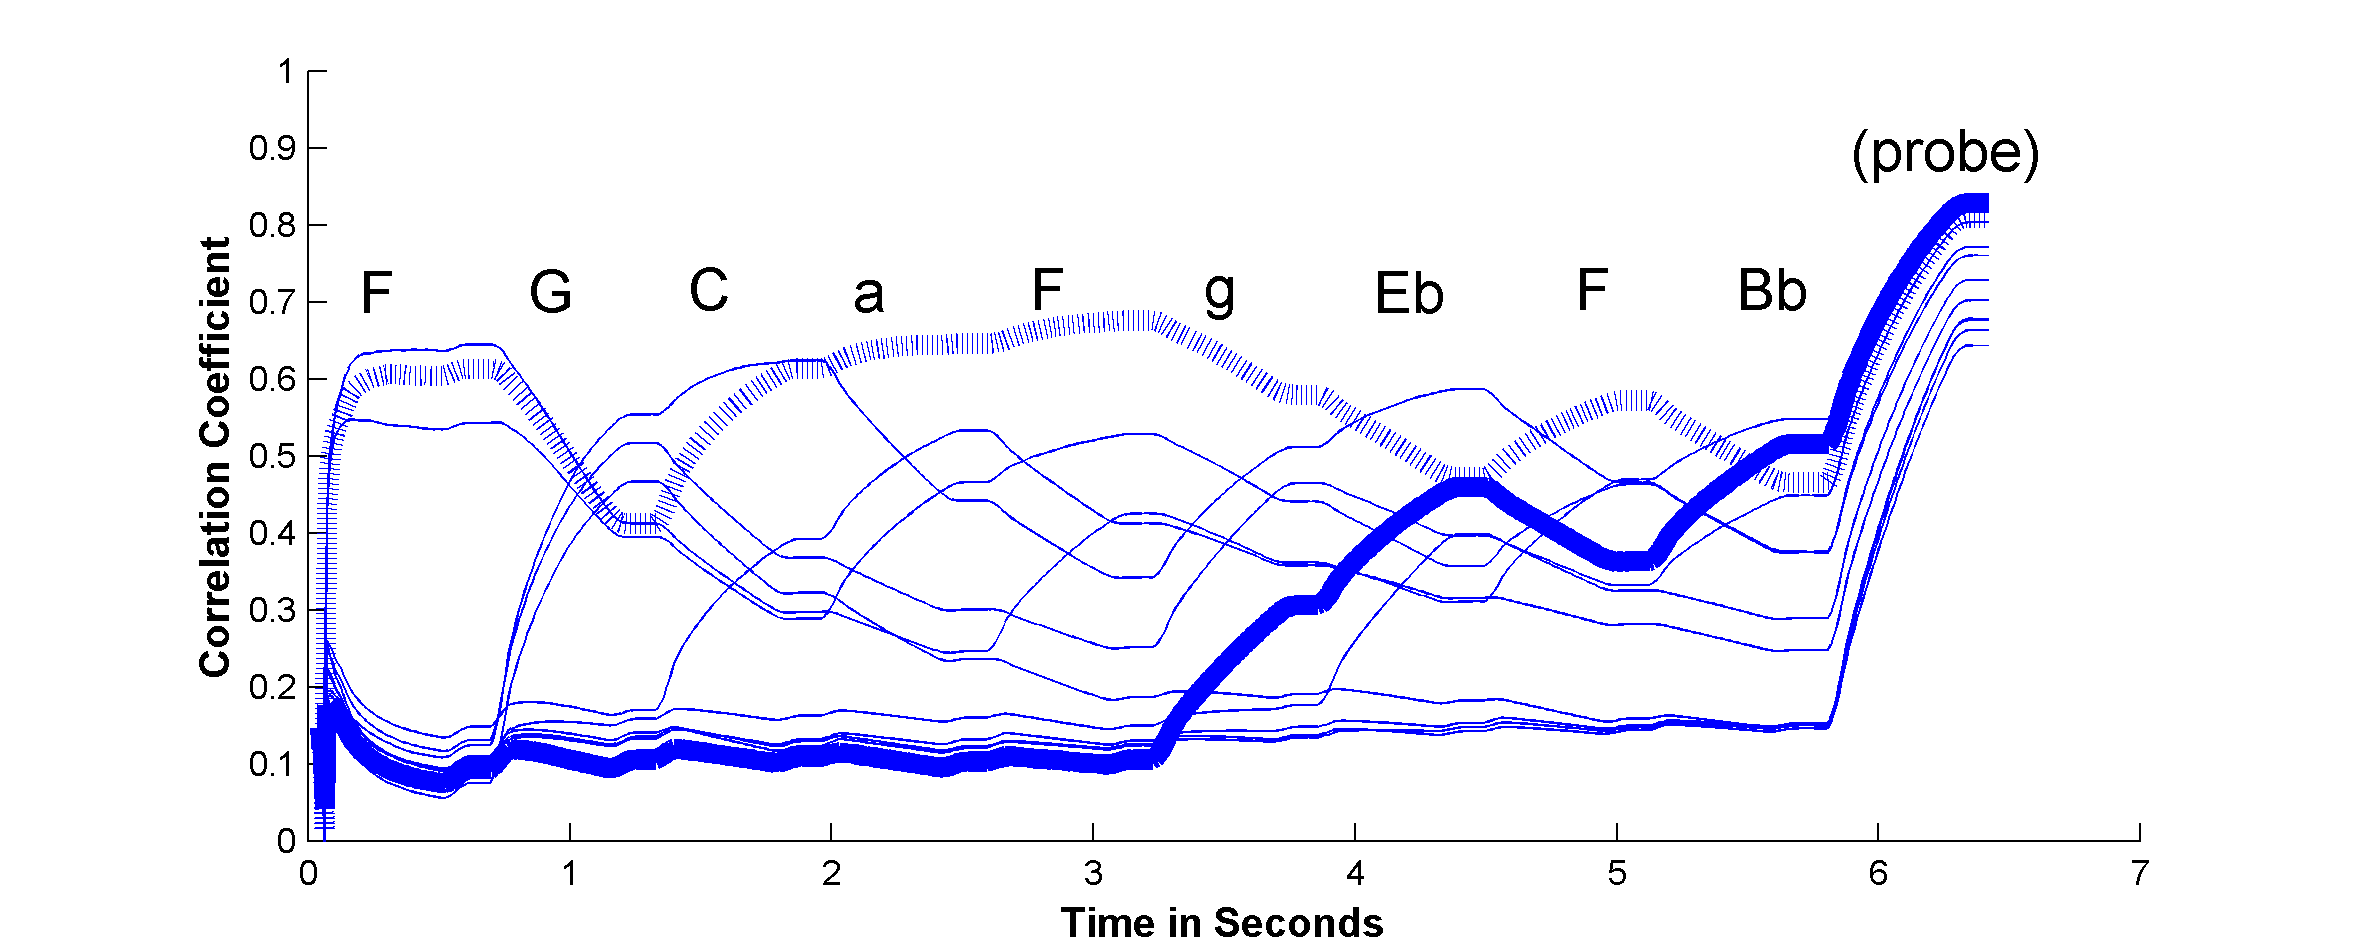
\includegraphics[width=\IPEMDefaultFigureWidth]{Graphics/TonalityDemoFig11}
    \caption {Stimulus-driven inferences (Method I) of chord sequence 4 used in Simulation II. The labels
    specify major and minor chords and are located at the time instances where they are
    introduced.
    The context-defining sequence is probed with 12 different probe tones. The stimulus-driven inference
    for each trial is plotted. The buildup and decay of the inferences depends on the echo of the global images
    ($T=1.5$). The dotted line represents the probe tone $c$, the solid line represents the probe tone $b\flat$}
    \label{Fig:TonalityDemoFig11}
\end{figure}

\begin{figure}[h]
    \centering
    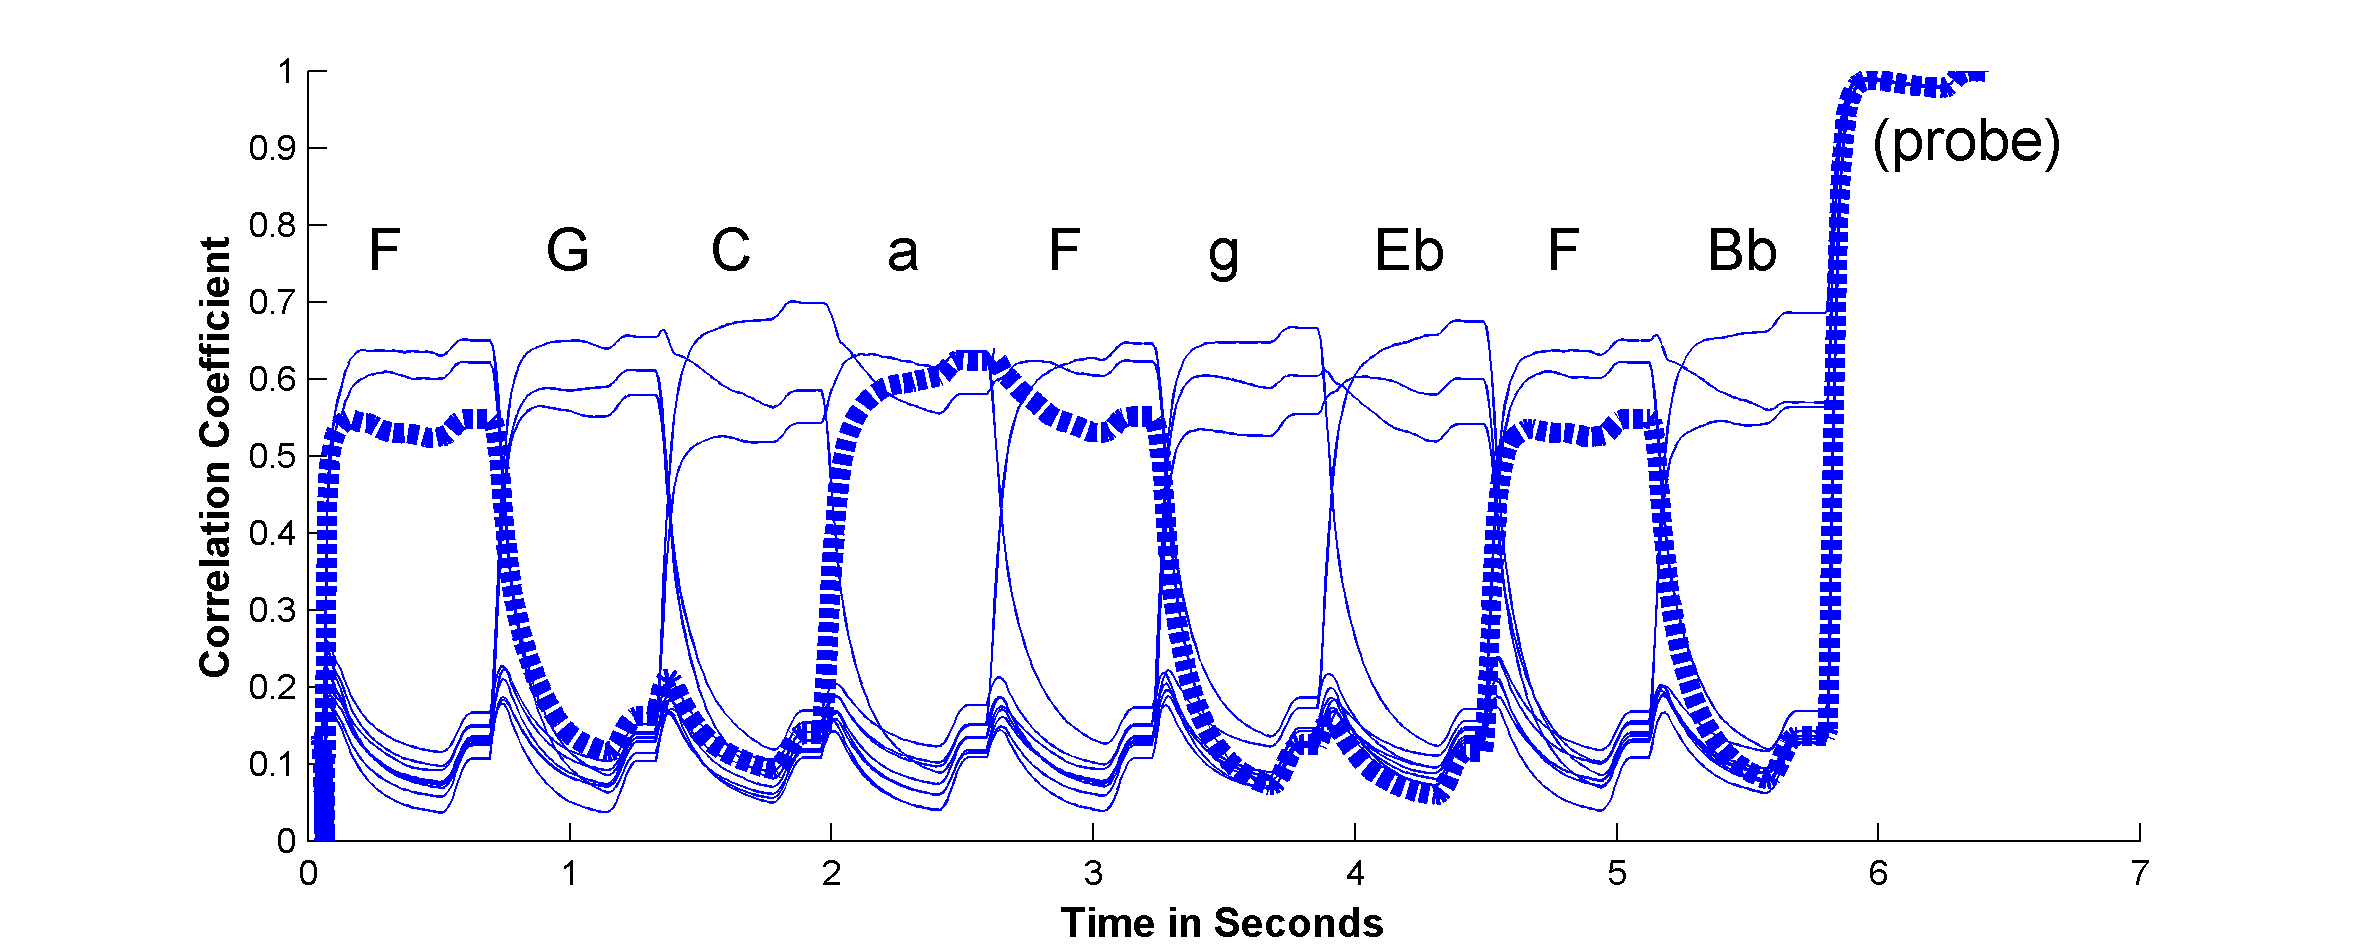
\includegraphics[width=\IPEMDefaultFigureWidth]{Graphics/TonalityDemoFig12}
    \caption{Stimulus-driven inferences (Method I)of chord sequence 4 used in Simulation II.
     The global images have the same echo as the local images ($T=0.1$). The dotted line represents the probe tone f.}
    \label{Fig:TonalityDemoFig12}
\end{figure}

The effects of echo are clearly visible in
Fig.~\ref{Fig:TonalityDemoFig11}. At the beginning of the
sequence, one gets the same profile for the F major chord as in
Fig.~\ref{Fig:TonalityDemoFig12}. But the next chords, G major and
then C major lead to quite different profiles, owing to the effect
of the echo. The dotted line shows the correlation with the probe
tone $c$, the tonic of the first key, the full line shows the
correlation with the probe tone $b\flat$, the tonic of the second
key. Shuffling chords around may have an effect on the resulting
profile. Certain chord progressions will prevent certain pitches
to pop up, while other chord progressions will favor other pitches
in the profile. But the echo takes into account the temporal order
of the chords, provided that it is within the limits of the half
decay time.

\subsection{Results and discussion}
% --------------------------------------------------------------------------------
Using the same stimuli as in Experiment I and Experiment II of
Krumhansl and Kessler \cite{KrumhanslKessler:82}, the short-term
memory model produces a good fit with the data. A comparison of
the key profiles of Simulation I with those obtained in Krumhansl
and Kessler's Experiment I gives a correlation of 0.848 for the
major key, and 0.825 for the minor key. The echo, or half decay
time, of the global image, which determines the content of the
context-defining sequence, was determined to be about 1.5 seconds.
Using this echo, Simulation II aimed at repeating Krumhansl and
Kessler's Experiment II in which the dynamic aspects of key
sensitivity were investigated.

\subsubsection*{Simulation I}
The results of Simulation I are summarized in Table
\ref{table_three}.
\begin{table}[!h]
\footnotesize
\begin{tabular}{lllllll}
T (=echo) & 1 vs 7+8+9 & 2 vs 10+11+12& 3 vs 7+8+9 & 4. vs
10+11+12 & KKMajor & KKMinor\\ \hline 0.2 & 0.989
&0.987&1.000&1.000&-0.519&-0.087 \\ 0.4 & 0.454& 0.531& 0.895&
0.891& 0.264& 0.493 \\ 0.6 & 0.258& 0.309& 0.907& 0.917& 0.771&
0.808 \\ 0.8& 0.390& 0.408& 0.891& 0.909& 0.809& 0.812 \\ 1
&0.509& 0.514& 0.872& 0.891& 0.827& 0.817 \\
1.2&0.603&0.601&0.855& 0.875& 0.838& 0.821 \\ 1.4& 0.672& 0.667&
0.841& 0.861& 0.845& 0.824 \\ 1.6&0.720& 0.714& 0.829& 0.850&
0.851& 0.826 \\ 1.8&0.755& 0.748& 0.820& 0.840& 0.855& 0.828 \\
2&0.780& 0.772& 0.813& 0.832& 0.858& 0.829 \\ 2.2&0.799& 0.790&
0.806& 0.826& 0.860& 0.830 \\ 2.4&0.813& 0.803& 0.801& 0.820&
0.863& 0.831 \\ 2.6 &0.824& 0.814& 0.796& 0.815& 0.864& 0.831 \\
2.8&0.831& 0.821& 0.792& 0.811& 0.866& 0.832 \\ 3&0.838& 0.827&
0.789& 0.807& 0.867& 0.832 \\ 3.2&0.843& 0.832& 0.786& 0.804&
0.868& 0.833 \\ 3.4&0.847& 0.836& 0.783& 0.801& 0.869& 0.833 \\
3.6&0.851& 0.839& 0.780& 0.798& 0.870& 0.833 \\ 3.8&0.853& 0.842&
0.778& 0.796& 0.870& 0.834 \\ 4&0.856& 0.844& 0.776& 0.794& 0.871&
0.834 \\ 4.2&0.858& 0.846& 0.775 &0.792& 0.871& 0.834 \\
4.4&0.860& 0.847& 0.773& 0.790& 0.872& 0.834 \\ 4.6&0.861& 0.849&
0.771& 0.788& 0.872& 0.834 \\ 4.8&0.862& 0.850& 0.770& 0.787&
0.873& 0.835 \\ 5&0.863&0.851&0.768&0.786&0.873&0.835 \\
\end{tabular}
\caption{The effect of changing the echo ($T$) of the global
images on profiles} \label{table_three}
\end{table}

The left column contains the half decay time $T$ of the global
images (the local images have a constant echo of $T=0.1$), the
first column reports the averaged correlation of the profile of
sequence 1 with the profile of sequences 7, 8, and 9. The second
column contains the average correlations of the profiles of
sequence 2 with those of sequences 10, 11, and 12, the third
column of 3 with 7, 8, 9, and the fourth of 4 with 10, 11, 12. The
last two columns contain the correlations of the major and minor
key profiles of Experiment I with those of Simulation I.

At $T=0.2$ the effect of the tonal context can be neglected. Hence
one gets high correlations between the profiles, but very low
correlations with the key profiles.  At $T=0.4$ the effect of
context is growing, but the local effects are still dominating.
For $T > 0.4$ the effect of context becomes visible and three
general trends can be distinguished:
\begin{itemize}
\item
The scale becomes more similar to the cadences, both for major and
minor.
\item
The chords become less similar to the cadences, both for major and
minor.
\item
The key profiles become more similar.
\end{itemize}
The trend can be explained in terms of the increasing contribution
of the tonic of the scale when $T$ increases. Taking into account
the data of Krumhansl and Kessler, who observed a less good
correlation with the scales than with the chords, the optimal echo
for global images is taken to be $T=1.5$. The effect is shown in
Fig.~\ref{Fig:TonalityDemoFig9}, where $T=4$, all other parameters
being equal.
\begin{figure}[h]
    \centering
    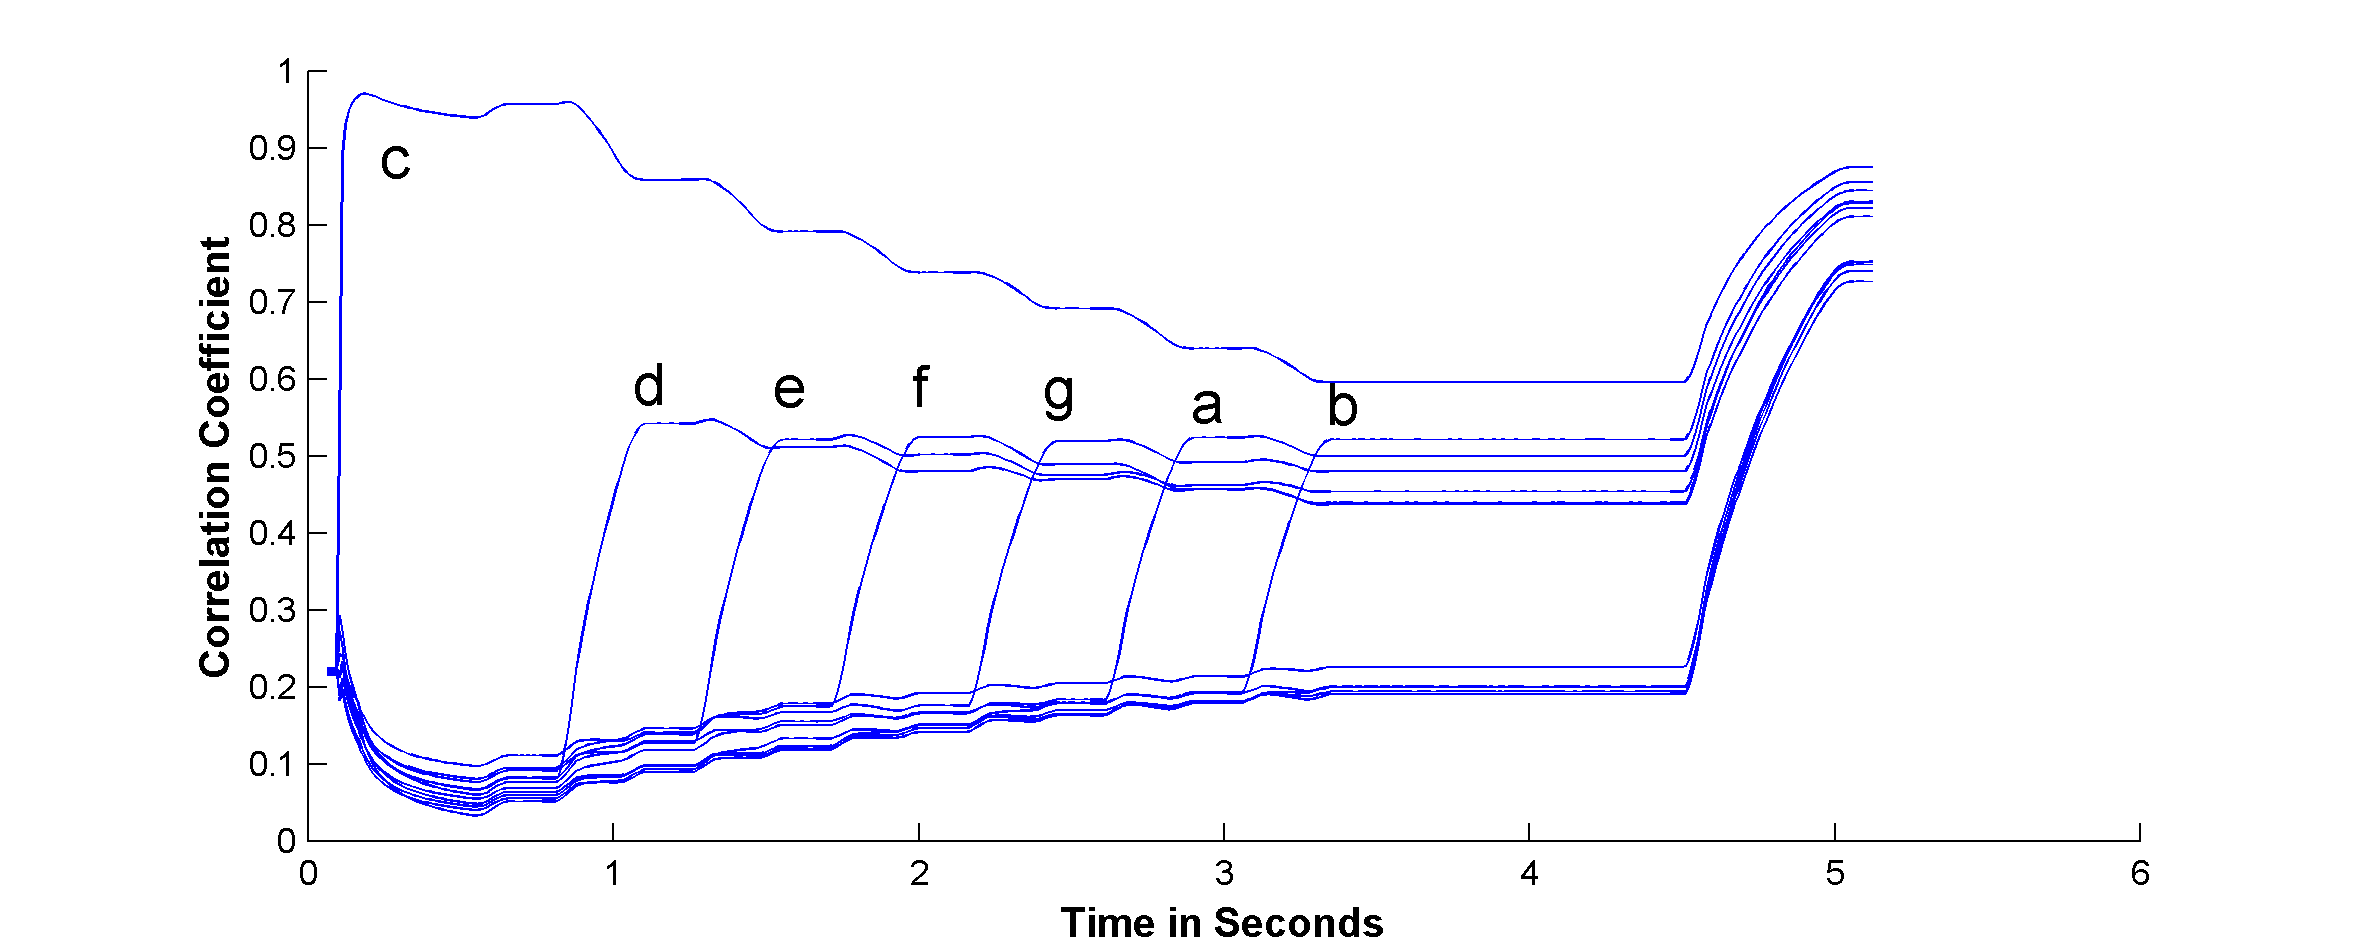
\includegraphics[width=\IPEMDefaultFigureWidth]{Graphics/TonalityDemoFig9}
    \caption{Stimulus-driven inference of the ascending C-major diatonic,
     using an echo of T=4 for the global images.}
    \label{Fig:TonalityDemoFig9}
\end{figure}

\subsubsection*{Simulation II}
The results of Simulation II Method I are summarized in five
graphs shown in Fig.~\ref{Fig:TonalityDemoFig100}.\\

Method I gives a useful insight in how the profiles are build up
during the temporal deployment of the chord sequence but the
actual build up of the profile should not be taken into
consideration when data are compared with the probe tone ratings.
What actually matters in that case is the snapshot taken at the
end of each trial of the chord sequence. This can be obtained with
either Method I or Method II. Fig.~\ref{Fig:TonalityDemoFig100}
shows the results when the average correlations are taken at the
end of each chord, for the nine chords in the
sequence.\\

\begin{figure}[!h]
    \centering
    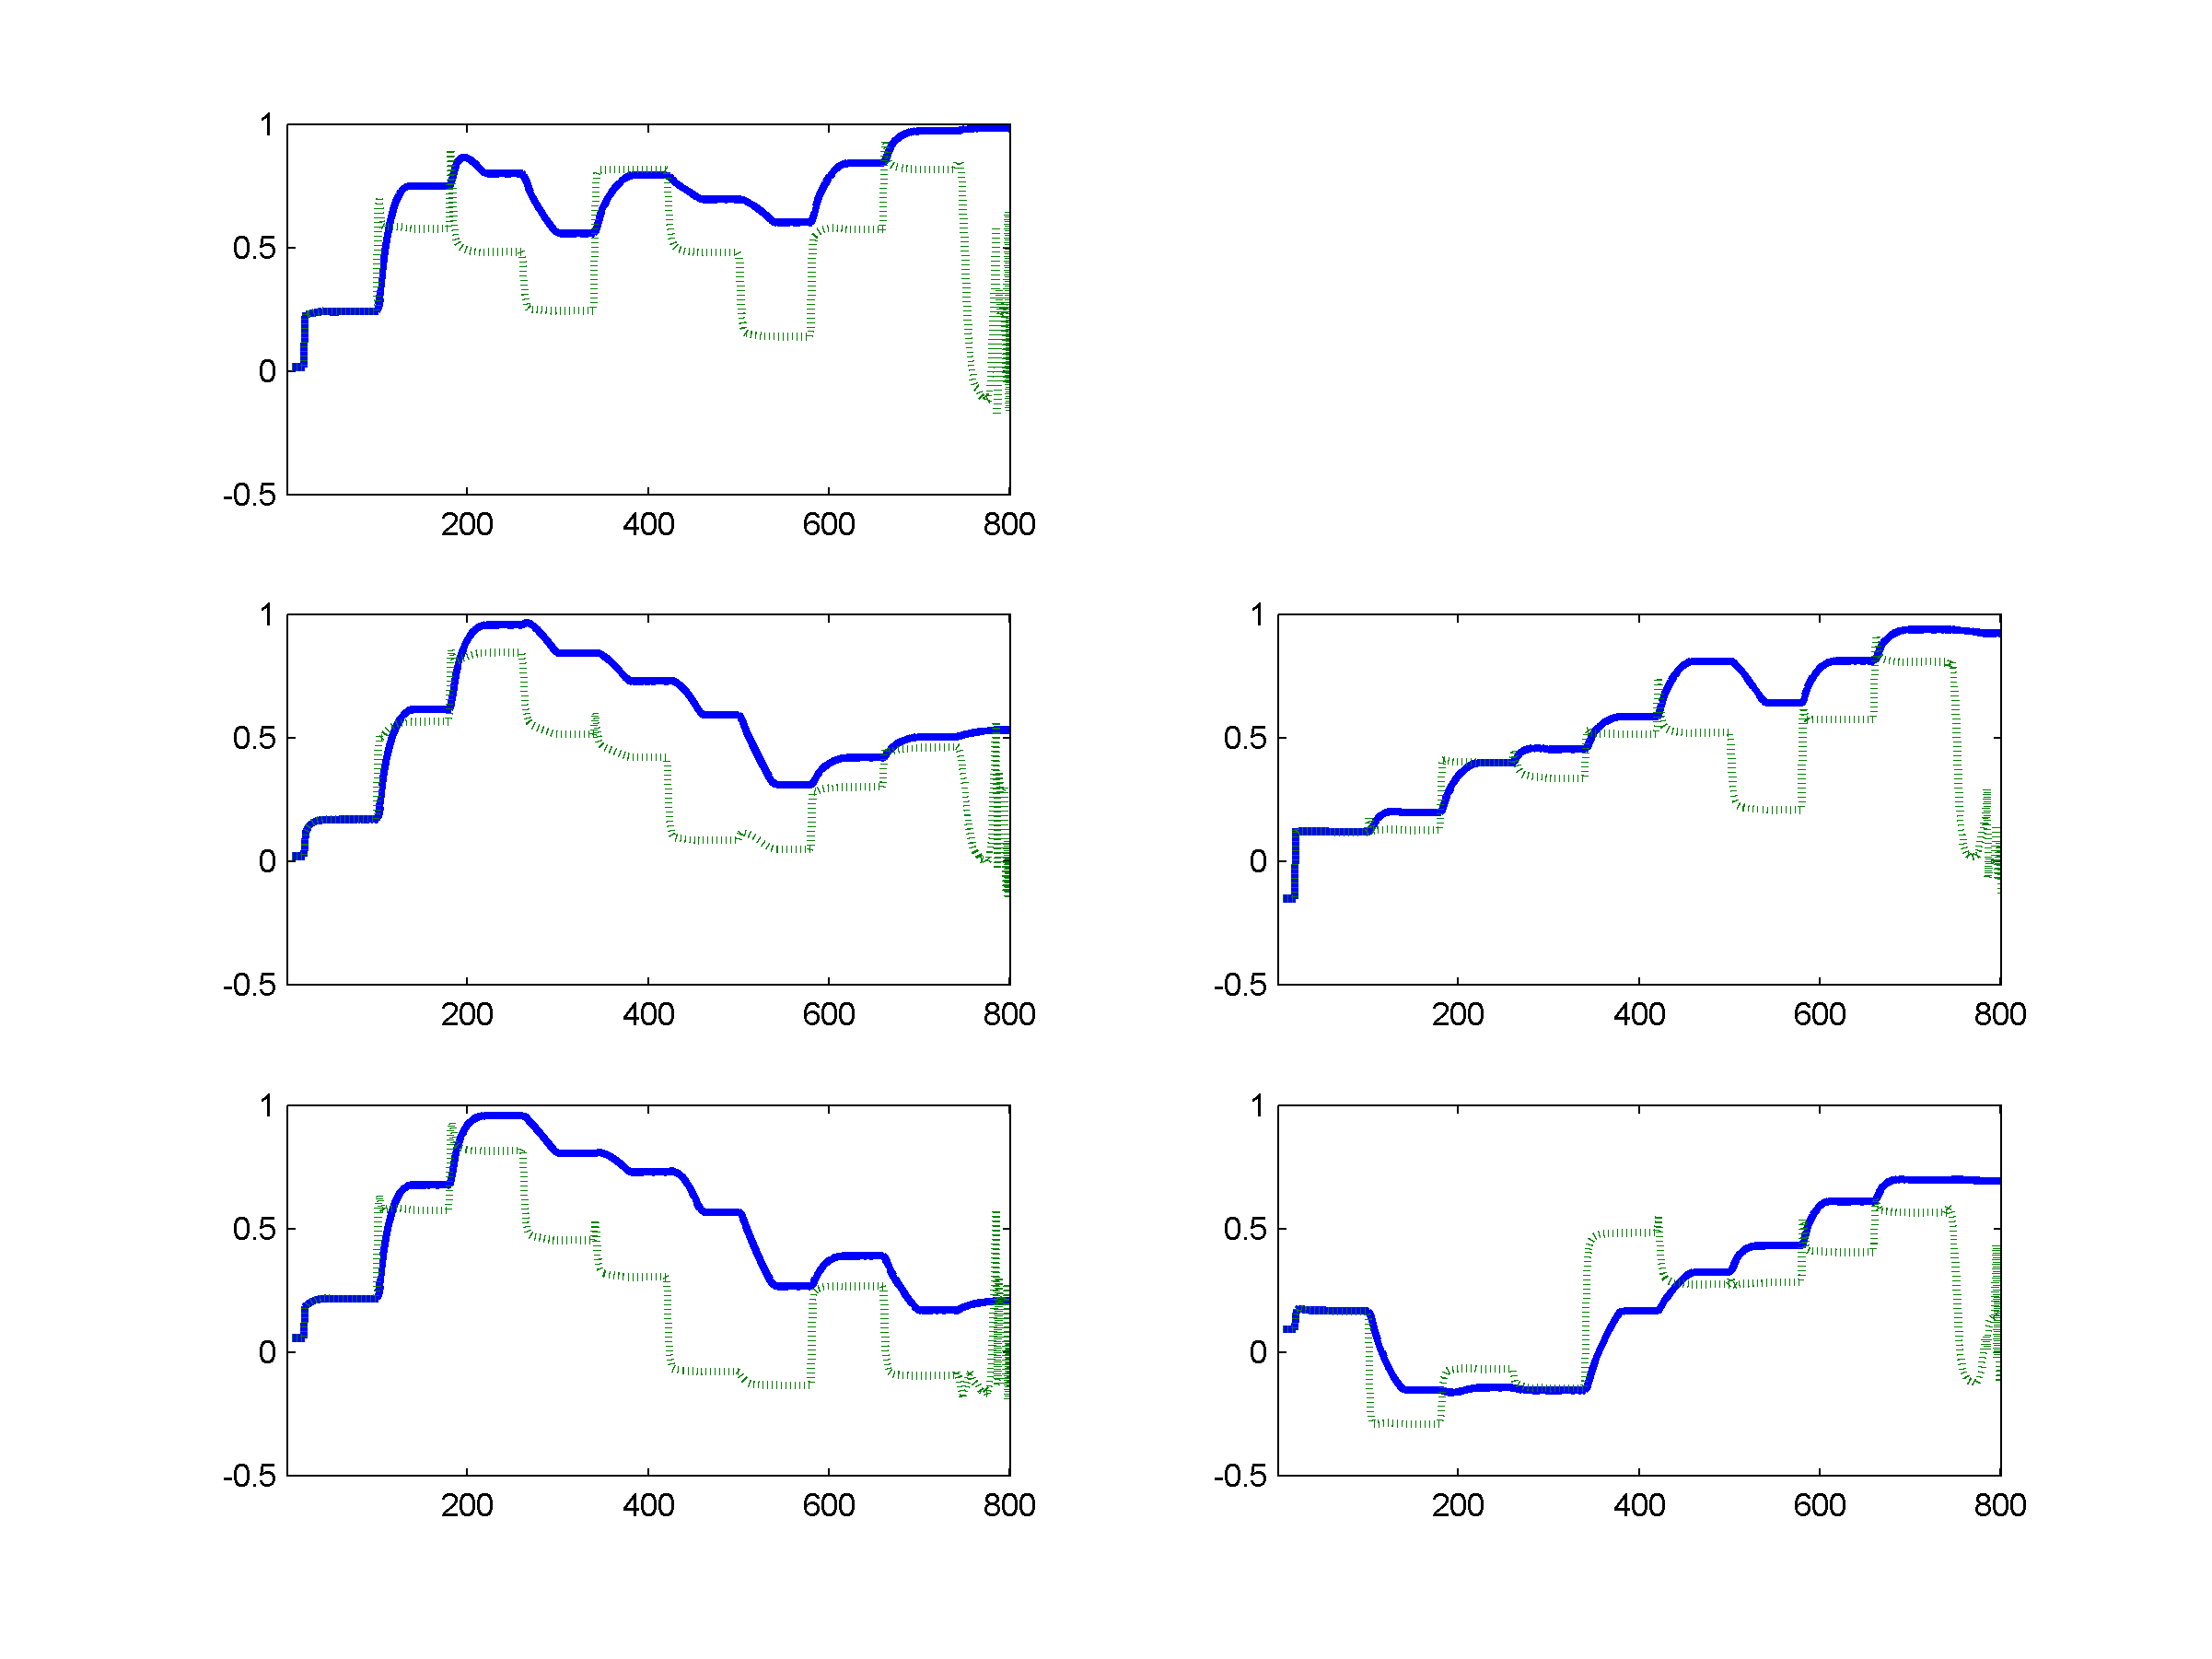
\includegraphics[width=\IPEMDefaultFigureWidth]{Graphics/TonalityDemoFig100}
    \caption{Results of Simulation II. The horizontal axis represents time in hundreds of seconds. The
    vertical axis is the correlation.The average correlations are
    taken at the end of each chord, for the nine chords in the
    sequences. The buildup effect of the local profiles now
    disappears.}
    \label{Fig:TonalityDemoFig100}
\end{figure}

\begin{figure}[]
    \centering
    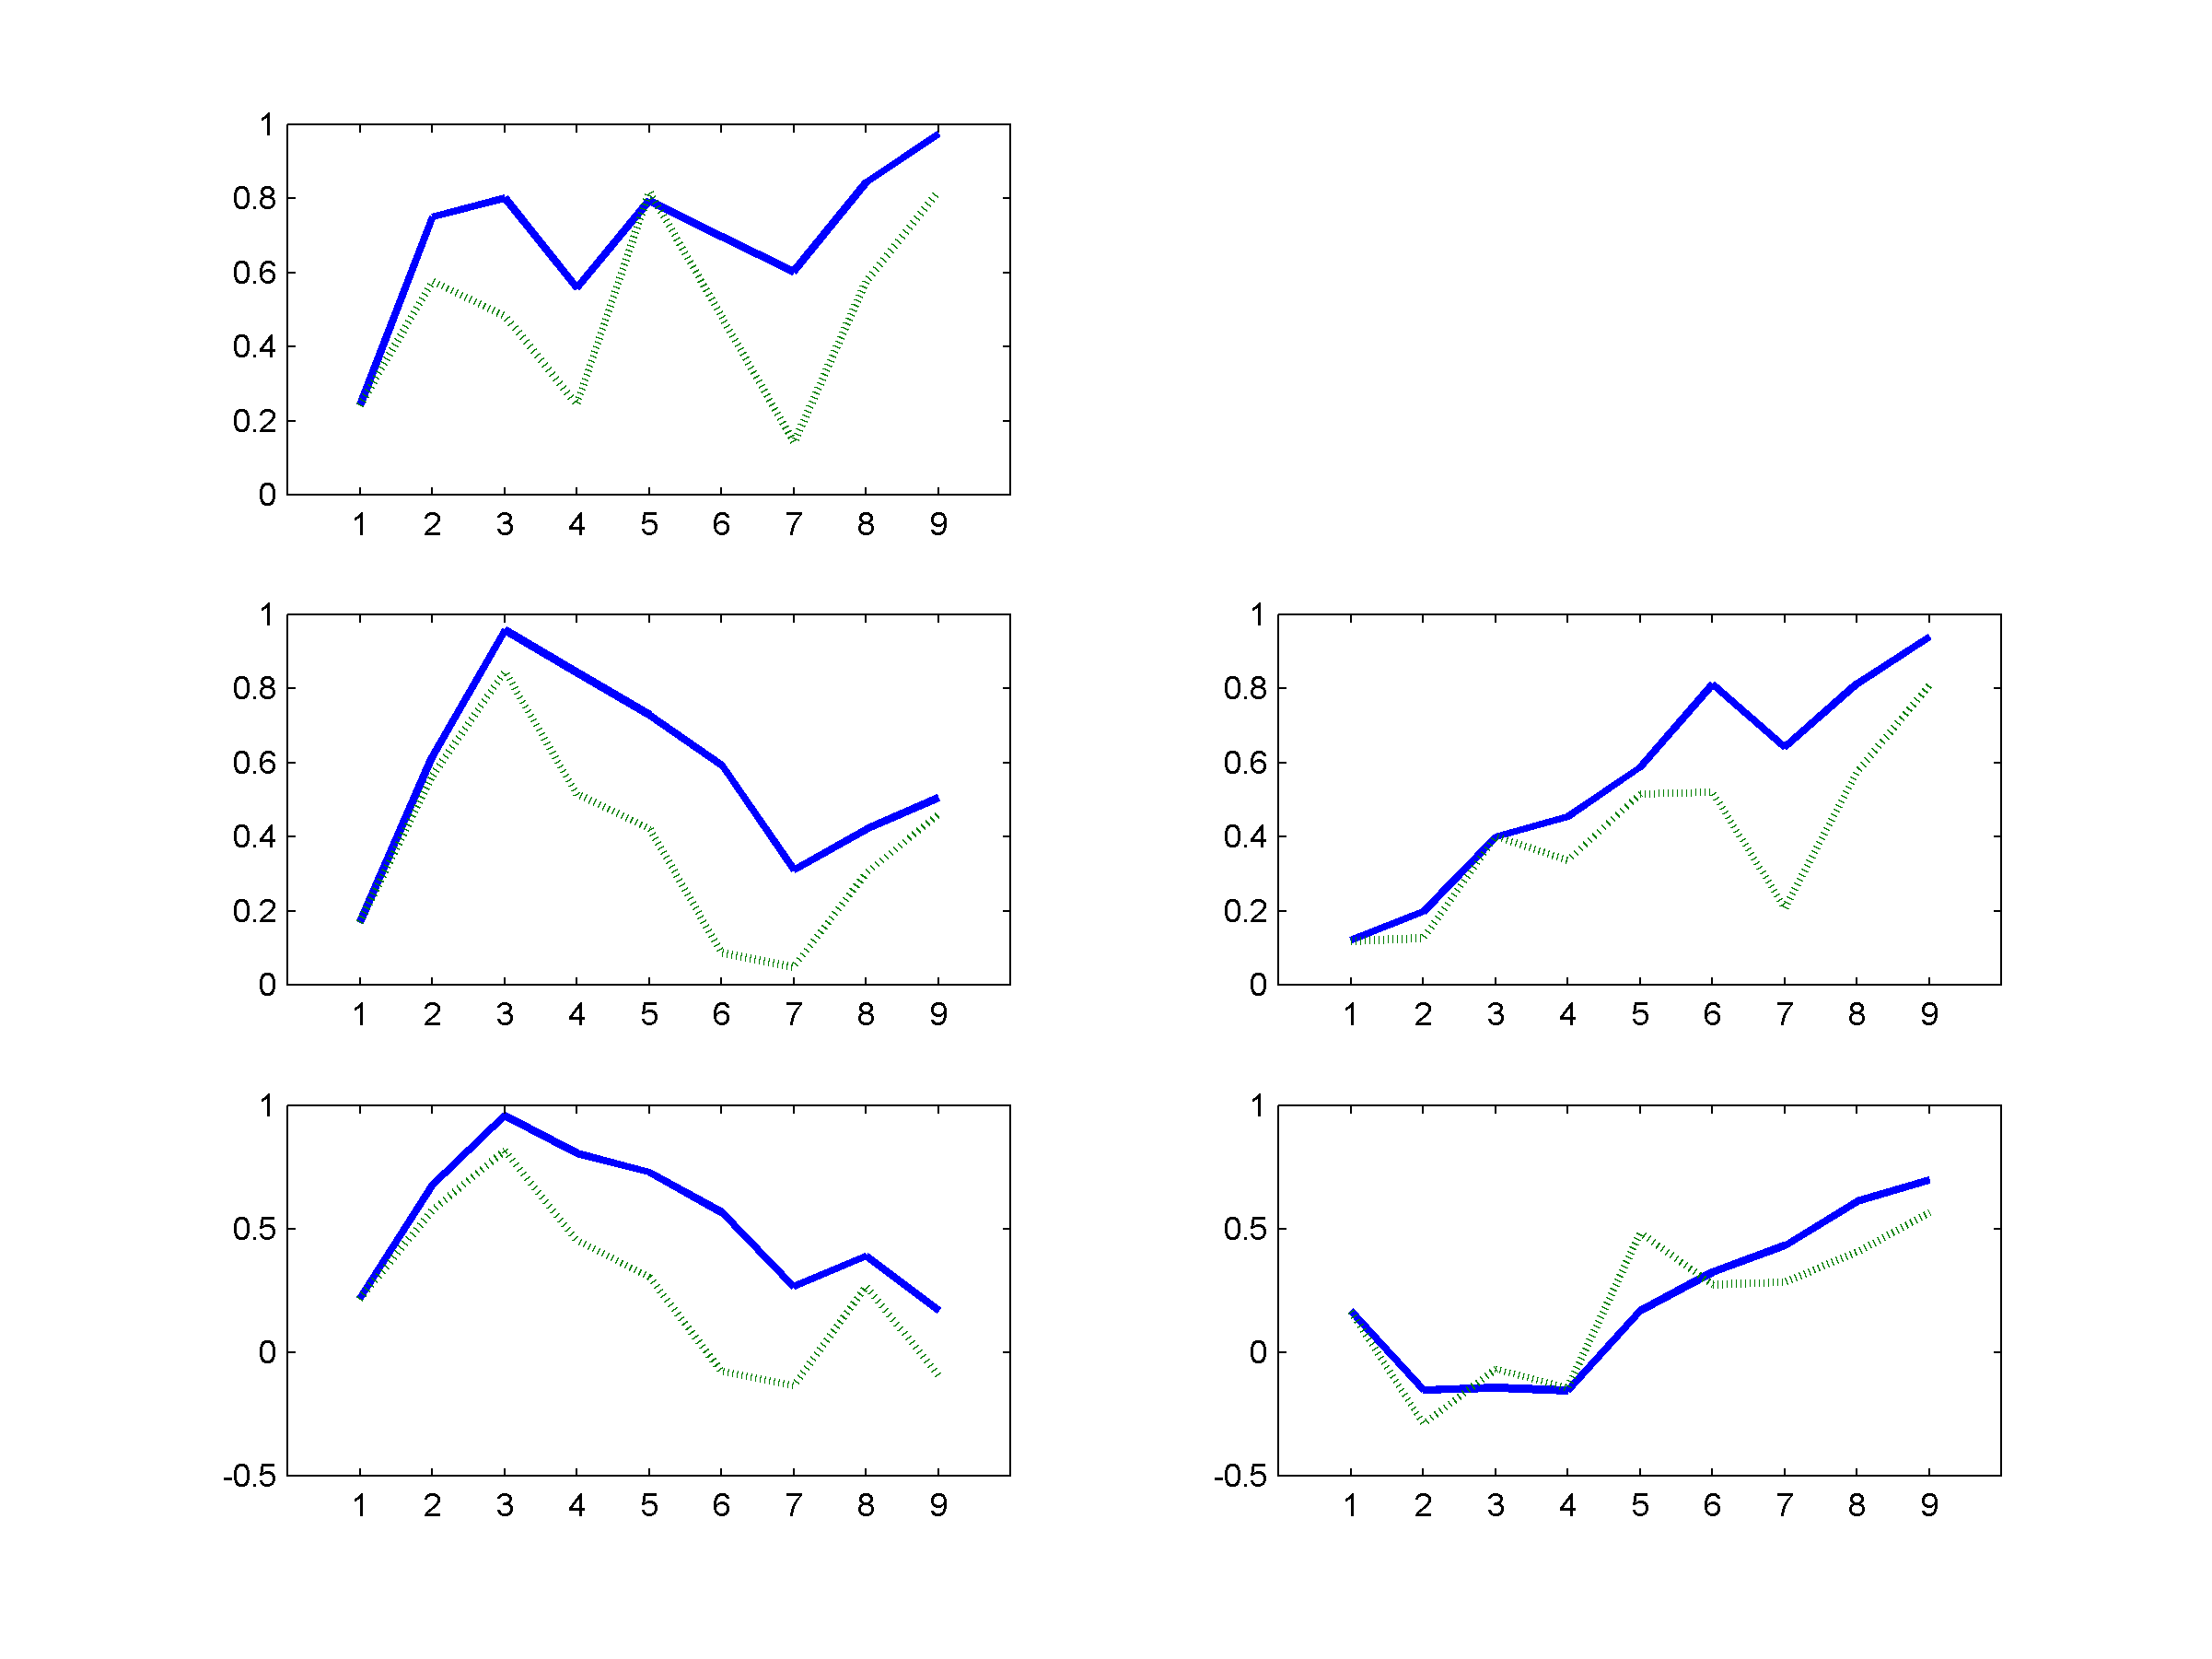
\includegraphics[width=\IPEMDefaultFigureWidth]{Graphics/TonalityDemoFig101}
    \caption{Results of Simulation II. Same graphs as previous figure, but the points
    at the end of each chord have been selected}
    \label{Fig:TonalityDemoFig101}
\end{figure}

The data of Experiment II are summarized as follows:
\begin{itemize}
\item
    The full line in the top left figure represents the average
    correlation-sequence for chord sequences 1 and 2. These chord
    sequences have no modulation, hence, the correlation-sequence for
    the first key is identical to the correlation-sequence for the
    second key. The data therefore collapse to a single figure.
\item
    The full lines in both middle figures represent the average
    correlation-sequences for chord sequences 3, 5, 7, 9 and 10. These
    chord sequences have a modulation between closely related keys.
    Given the two different keys, the results are split up in two
    figures, one left and one right figure. The full line on the left
    figure contains the averaged correlation-sequence with the first
    key. The full line on the right figure contains the averaged
    correlation-sequence with the second key.
\item
    The full lines of the bottom figures represent the average
    correlation-sequences for the chord sequences 4, 6, and 8. These
    chord sequences have a modulation between distant keys. The full
    line on the left figure contains the averaged correlation-sequence
    with the first key. The full line on the right figure contains the
    averaged correlation-sequence with the second key.
\end{itemize}
The dashed line in each of the left-sided figures represents the
averaged correlation between the profile of the individual chords
and the profile of the first key, at each of the nine steps. The
dashed line in each of the right-sided figures represents the
averaged correlation between the profile of the individual chords
and the profile of the second key, at each of the nine steps. For
example, in the top left figure, the dashed line of the first
point is the average of two correlations, in particular the
correlation between the profile of the F major chord, and the C
major key profile, and the correlation between the profile of the
F minor chord and the C minor key profile. (The chord profiles and
the key profiles used to calculate the dashed line were all
obtained in Experiment I.) The correlations between the individual
chord profiles and the key profiles predict how strongly each
chord in isolation would be expected to be related to the intended
key of the sequence and, thus, serve as a baseline against which
the strength of the intended key can be compared. There is a
striking similarity with the results of Krumhansl and Kessler
Experiment II. The correlation ranges show a good agreement for
both lowest and highest values. There is a small difference in
the comparison of profiles to the first key (=left colomn
figures). The listeners seem to sense the key already after the
second chord, which is not the case in the simulation, where the
correlations corresponding to the global and local images are
almost similar for the first two chords of the sequence.

% --------------------------------------------------------------------------------
